\ifpdf
	\graphicspath{{3/pic/PNG/}{3/pic/PDF/}{3/pic/}}
\else
	\graphicspath{{3/pic/EPS/}{3/pic/}}
\fi

\chapter{Neutron transport approximations}\label{chap:nte-methods}

As mentioned in the introductory chapter, we will focus on deterministic methods for solving the NTE, requiring proper
discretization of \eqref{eq1} and solution of the resulting system of algebraic equations.
In the following sections, we review some of the most widely used semi-discretizations with respect to energy, angle and
spatial variables and put them into a unified Hilbert space projection framework. We finish this chapter with a general
discussion on solving the associated large sparse systems of algebraic equations and a review of adaptive approaches to
these discretizations (some of which will be later developed in \cref{chap:hermes}). We will focus on the fixed-source
problem, whose solution is a neccessary part in practically all numerical methods for solving the generalized eigenvalue
problem \eqref{eq:critical}.

\myparagraph{Notation conventions}
Concerning fonts and subscripts/superscripts, we will generally use the following conventions (wherever exception will
be needed, it will be clearly stated):
\begin{itemize}
  \item $\mathbf{f}$ $\ldots$ column vector with numerical values ($\mathbf{f}\in\R[N]$ for some $N\in\mathbb{N}$);
  \item $f_n$ or $[\mathbf{f}]_n$ $\ldots$ components of $\mathbf{f}$;
  \item $\mathbf{A}$ $\ldots$ matrix with numerical values ($\mathbf{A}\in\R[M\times N]$, $M,N\in\mathbb{N}$);
  also, $\mathbf{A}(\br)$ will denote matrix-valued function with elements being functions defined in~$\VV$;
  \item $A_{ij}$ or $[\mathbf{A}]_{ij}$ $\ldots$ elements of $\mathbf{A}$;
  \item upshape $\mathrm{F}$ (including $\Psi$, $\Phi$) $\ldots$ vector-valued function $\VV\to\R[N]$,
  $N\in\mathbb{N}$; as an exception, $\bn(\br)$ denotes as before the vector-valued function representing unit outward
  normal field of $\pV$;
  \item $f_n$ or $[\mathrm{F}]_n$ $\ldots$ components of $\mathrm{F}$\comment{ (we will not need to distinguish between
  components of $\mathrm{F}$ and $\mathbf{f}$ at the same place, so we use $f_n$ for both)};
  \item $A$ or calligraphic $\mathcal{A}$ $\ldots$ in the context of an operator acting on some vector space $V$, usual
  letters will be used for transport operators introduced in previous chapter, while calligraphic letters for general  
  operators;
%   \item $[A]_{ij}$ $\ldots$ sometimes we will use matrix operators acting on $\mathrm{F}\in V^N$; then 
%   $$
%   	[A \mathrm{F}]_{i} = \sum_{j=1}^N [A]_{ij} f_j
%   $$
  \item $s = \{c_k\}_{k=1}^N \equiv \{c_k\}_\idxset{N}$;
  \item $\col s$ $\ldots$ column vector with entries $c_1,c_2,\ldots,c_N$;
  \item $\diag s$ $\ldots$ diagonal matrix whose diagonal is given by elements of $s$;
  \item $f_{(i)}$ $\ldots$ $i$-th iterate in an iteration process.
\end{itemize}
So with this notation, we have, for instance, $\mathrm{F} = \col \{f_n\}_N$ with each $f_n$ being a function from some
space $V_n$.
\mbox{}\\

To facilitate comparison of the results with literature, we also neglect inelastic scattering (i.e., put $\eta \equiv
1$). The scattering component of the collision kernel (first relation in \eqref{eq:ddifxs}) then becomes
\begin{equation}\label{eq:ddifxs2}
	\sigma_s(\br, E) =
\intE[']{\Emin}{\Emax}{\intA[']{\sigma_s(\br,\bomega'\cdot\bomega, E'\sla E)}}.
\end{equation}

\section{Approximation of energetic dependence}\label{sec:MG}

The continuous dependence on energy, $\psi = \psi(\cdot, E)$, is typically resolved by the so called \textit{multigroup
approximation}. In this approximation, the interval of neutron energies is divided as follows:
$$
\begin{multlined}
  \bigl[\Emin,\Emax] = \bigl[E^{G}-\dEh{G},E^{G}+\dEh{G}\bigr]\cup \ldots\\
  \ldots \cup \bigl[E^{g}-\dEh{g}, E^{g}+\dEh{g}\bigr] \cup \ldots \cup
  \bigl[E^1-\dEh{1},E^{1}+\dEh{1}\bigr],
\end{multlined} 
$$
and equations \eqrefs{eq1}{eq:nte3} are integrated over each energy group range 
\linebreak
\mbox{$\bigl[E^{g}-\dEh{g}, E^{g}+\dEh{g}\bigr]$}.
\begin{remark}
Note that the energy intervals (groups) are traditionally numbered in a descending order, i.e. a group with larger index
contains lower energies than a group with lesser index; also, the group index is traditionally placed in superscript. 
\end{remark}
The NTE \eqref{eq1} is thus transformed into a finite system of integro-differential equations, each
governing the flux of neutrons with energies within a particular range (in this context called \textit{group}):
\begin{equation}\label{eq:psi-MG}
\begin{multlined}
  \psi^g(\br, \bomega) = \frac{1}{\Delta E^{g}}\int_{g}\psi(\br, \bomega, E),\d{E} \equiv
  \frac{1}{\Delta E^{g}}\int_{E^g-\Delta E^{g}/2}^{E^g+\Delta E^{g}/2}\psi(\br, \bomega, E),\d{E},\\ g = 1, 2,\ldots
  G.
\end{multlined}
\end{equation} 
This conventional procedure leads to the following set of $G$ coupled neutron transport equations
\begin{equation}\label{eq:mg}
	\left\{
	  \begin{aligned}
      &T_G\{\psi^g\}_G = \{q^g\}_G,\\
      &\Dom{T_G} = \bigl\{\{\psi^g\}_G\in \bigl[\Hp(\XE)\bigr]^G,\ \psi^g\vert_{\pXE[-]} = 0,\ g = 1,\ldots,G\bigr\},
    \end{aligned}
  \right.\\[.2em]
\end{equation}
where
$$
	\XE \coloneqq \{(\br,\bomega):\ \br\in \VV\subset\R[3], \bomega\in \Sphere\}
$$
is the 5-dimensional subspace of $X$ (i.e., the norm in $\Hp(\XE)$ is defined as
in \eqref{eq:Hp} but only using double integrals over $\VV\times\Sphere$) and analogously for $\pXE$.
The multigroup transport operator has the following form:
\begin{equation*}
\begin{gathered}
    T_G\{\psi^g\}_G = \left\{\left(A + \Sigma_r^g\right)\psi^g - \summ{g'=1,g'\neq g}{G}
    K^{gg'}\psi^{g'}\right\}_G,\\
    \bigl(\Sigma_r^g\psi^g\bigr)(\br,\bomega) = \sigma_t^g(\br)\psi^g(\br,\bomega) - \intA[']{\kappa^{g\sla
    g}(\br,\bomega\cdot\bomega')\psi^g(\br,\bomega')},\\ \bigl(K^{gg'}\psi^{g'}\bigr)(\br,\bomega) =
    \intA[']{\kappa^{g\sla g'}(\br,\bomega\cdot\bomega')\psi^{g'}(\br,\bomega')}
\end{gathered}
\end{equation*}
where the terms with superscript $g$ or $g'$ represent quantities suitably averaged over 
\mbox{$\bigl[E^{g}-\dEh{g}, E^{g}+\dEh{g}\bigr]$}, e.g. $k^{g\sla g'}$ is (in theory) obtained as
\begin{equation}\label{eq:mg-kappa}
	\kappa^{g\sla g'}(\br,\bomega\cdot\bomega') = \frac{\int_{g}\int_{g'} \kappa(\br,\bomega\cdot\bomega',E \sla
	E')\psi(\br,\bomega,E')\,\d{E'}\d{E}}{\int_{g}\psi(\br, \bomega', E)\,\d{E}}.
\end{equation}
It is customary to move the \textit{self-scattering} (diagonal) part of the
collision operator to the reaction operator. Since the reactions in which energetic distribution of both the incoming 
and outgoing neutrons lies within the same group are included in both $\sigma_t$ and $\kappa$  (compare equations
\eqref{eq:ddifxs} and \eqref{eq:st}), this transformation makes $\Sigma_r^g\psi^g$ represent the actual rate of neutron
removal from the group, while $K^{gg'}\psi^{g'}$ the rate of neutron addition to that group. Results about unique
solvability presented in previous chapter carry over to the multigroup setting by considering a counting measure on the
set $\{E^G,\ldots,E^1\}$ instead of the continuous Lebesgue measure $\d{E}$ \cite[Chap. XXI \S 2]{DautrayLions}.

\subsection{Multigroup data}
Although the multigroup system of neutron transport equations has a relatively simple form, finding an optimal grouping
of energies and determining the associated group-averaged coefficients is not an easy task in most practical
applications because of the highly complicated energetic dependence of nuclear processes, as illustrated by the typical
dependence of the (microscopic) fission cross-section of \isotope[235][92]{U} in the so-called resonance range of
energies and corresponding multigroup approximation in Fig. \ref{fig:xs}.
\begin{figure}[htp]
\begin{center}
  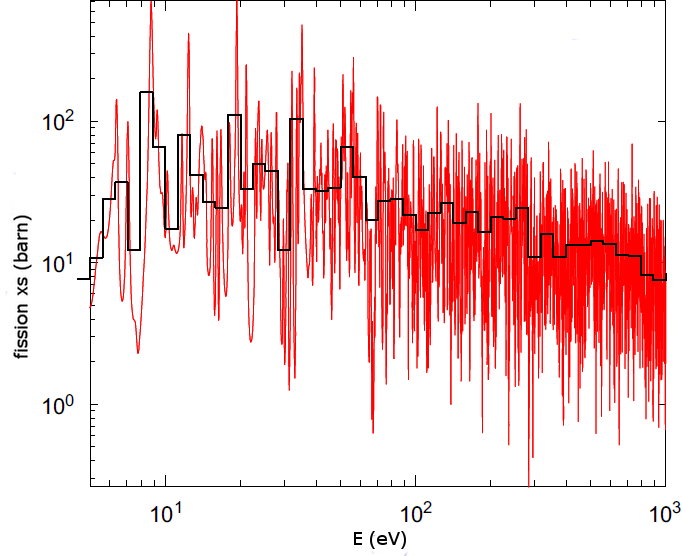
\includegraphics[scale=.4]{U235fg}
  \caption{Microscopic fission cross-section of U235}
  \label{fig:xs}
\end{center}
\end{figure}
Suitable approximation of the unknown exact solution in \eqref{eq:mg-kappa} is also highly non-trivial, albeit essential
for the success of the multigroup method. Even though an alternative to the finite-volume like approximation
\eqref{eq:psi-MG} has been proposed recently  in \cite{Douglass} -- using Galerkin projection of angular flux onto a
space of functions supported over subregions of the energy range (a finite-element like approach) --  the multigroup 
approximation still remains the most universally used approach to simplify the energetic dependence (see, e.g., 
\cite[Chap.~5]{Cacuci1} or \cite{Cho1}). However, we will not specifically address this issue and always assume that 
the multigroup coefficients appearing in the equations are given as input.
\begin{remark}{\textsc{Fission spectrum}}
In criticality problems, the set of multigroup data must include both parts of the collision kernel
$\kappa^{gg'}$, i.e. the cross-sections $\sigma_s^{gg'}$ and $\sigma_f^{gg'}$, as well as $\nu^{g'}$ and
$\chi^g$. Because of the rapid
decay of $\chi(E)$ for low energies (as neutrons are mostly emitted from fission with high energies) that are
nevertheless the most important for the cross-sections (as most interactions are likely to occur due to slowly moving
neutrons, at least in classical moderated reactors)\footnote{cf. \fref{fig:xs} and \fref{fig:spectrum} and notice the
different scaling on the horizontal axis}, there will typically be $\chi^g = 0$ for $g = G,G-1,\ldots,G-k$. The
group-discretized operator $F$ from \eqref{eq:FScrit} will therefore have a non-trivial null-space, leading ultimately
to a fully discrete generalized eigenproblem of type $\mat{A}\mat{x} = \lambda\mat{B}\mat{x}$ with singular $\mat{B}$.
\end{remark}


\subsection{Group source iteration}
A standard way of iterative solution of the multigroup system is the \textit{group source iteration}: for a given
initial approximation $\psi^g_{(0)}$, $g = 1,\ldots,G$, solve
\begin{myitemize}
  \item \textbf{for} i = 0,1,\ldots
  \begin{myitemize}
  \item \textbf{for} g = 1,\ldots,G
  \vspace*{-.5em}
	\begin{equation}\label{eq:MGGS}
		\left(A + \Sigma_r^g\right)\psi^g_{(i+1)} = \summ{g'\leq g-1}{} K^{gg'}\psi^{g'}_{(i+1)} + \summ{g' \geq g+1}{}
	  K^{gg'}\psi^{g'}_{(i)} + q^g
	\end{equation}  
 \end{myitemize}
\end{myitemize}
If we view the operator $T_G$ as a matrix operator acting on $\col \{\psi^g\}_G$, then we can interpret
this iteration as a Gauss-Seidel iteration for \eqref{eq:mg}, where $T_G$
has been split into its lower-triangular part $A + \Sigma_r^g - K^{gg'}$ ($g'\leq g$) and its upper triangular part 
$K^{gg'}$ ($g'> g$) and the lower triangular part is being inverted by forward substitution. Convergence of this scheme can become slow when the upper triangular part (representing neutron up-scattering
from lower energies to higher energies) is dominating. Therefore, when preparing the multigroup data, it is
advantageous to put an effort into finding such an energy grouping that minimizes the up-scattering (which is often
done in practice, as in e.g. \cite{mox-bench}).
\begin{remark}\label{rem:SI}
Here we assume that the
mono-energetic problem can be solved exactly. Approximations of angular dependence discussed in the following
section (like the $\SN$ method) may employ another iteration level to resolve angular
coupling of the within-group fluxes induced by collisions. This iteration is usually called just \textit{source
iteration} and can also become very slow if scattering of neutrons with given energy dominates their absorption (we will
return to this issue later in \sref{sec:SI}).
\end{remark}

Note that by employing the group source iteration, only a mono-energetic transport problem in group $g$ has to be
solved in each iteration, and if the differential part $A$ can be represented by a symmetric operator $\tilde A$ (as can be done for some of the second-order forms
described in \sref{sec:L2} or when suitable angular approximations like diffusion are being
used -- see \sref{sec:diffusion}), the problem would become symmetric with implications for efficient numerical
solution. In the remainder of this chapter, we will focus on the approximation of neutron flux in a single
group (index of which will be omitted), described by the corresponding within-group equation in which contributions from
other groups are encapsulated in the source term $\src$ (i.e., we will study the NTE on $\XE$). In order to simplify
notation, we will use just $X$ instead of $\XE$ when refering to the solution domain.

\section{Approximation of angular dependence}

Considerably larger number of methods have been proposed for approximating the angular dependence of neutron
flux. Many of them are still used and actively developed today as their characteristics make them more suitable for one
application area than other methods, which are preferred in different areas.

\subsection{Methods based on the integral form of NTE} \label{sec:lattice}
As a first example, we consider the class of
methods originally derived from the equivalent integral form of the NTE (see \sref{sec:advection}). Typical
representatives of this class are the method of collision probabilities or the method of characteristics (see e.g.
\cite{Cho2,Wu1,Hursin1,Petkov1,Sanchez1}). As the integral form of the NTE represents the global neutron balance over
the domain, the corresponding algebraic systems (obtained after spatial discretization) are full and
their solution demanding on computer resources. On the other hand, these methods quite naturally handle complex
geometries. Taking into consideration smaller geometric features of the domain, we are effectively coming from a
macroscopic scale to a mesoscopic range where the neutrons direction of motion as well as their kinetic energy become
more significant. High degree of spatial coupling and the requirement of fine resolution of angular and energetic
dependence does not make these methods suitable for whole-core reactor calculations.
However, these small-scale,
high-fidelity calculations\footnote{called \textit{lattice calculations} as they are typically performed on a single
representative subdomain of the core (one or several neighboring assemblies of fuel pins, or the fuel pin itself)
with reflective boundary conditions, simulating an infinite lattice of such subdomains} are indispensable for
generating appropriately averaged coefficients for the computationally more feasible larger scale calculations.
This \textit{spatial homogenization} and \textit{energy group condensation} (already mentioned in the previous
section), as these averaging procedures are traditionally called in nuclear engineering field, are employed by many existing whole-core simulators (see e.g.
\cite[Chap. 17]{Reuss1} or the review in first two sections of \cite{Sanchez7}). To simulate a long-term nuclear reactor
operation, it is furthermore neccessary to perform these procedures under varying physical conditions of the core and
generate many sets of averaged coefficients corresponding to these conditions.\comment{The code system
developed as part of author's involvement in the TACR project expects these coefficient sets on input, i.e., it is not
designed for lattice calculations.}

\subsection{Methods based on the integro-differential NTE}\label{sec:idNTE} 

More suitable for whole-core calculations are methods derived from the integro-differential
version of the NTE, eq.
\eqref{eq1}, which lead to sparse algebraic systems. The most successful and well-established are the method
of discrete ordinates ($\SN$) and the method of spherical harmonics ($\PN$).
Both arise from applying in the
angular domain a classical well known approach for constructing finite numerical
approximations of PDEs. \comment{Although in the final code, we ultimately use the lowest order approximation that can
be obtained equivalently from both approaches (the neutron diffusion model) we will briefly introduce the main ideas behind the
$\SN$ and $\PN$ methods and expose their most important properties in the next two subsections.} In the following
sections, we will briefly introduce the main ideas behind the $\SN$ and $\PN$ methods and expose their most
important properties. These properties are generally known, but their origin in mathematical structure of the
approximate forms is mostly overlooked in literature (a few exceptions will be cited below and in the corresponding
appendices). 

We will also interpret both methods as restrictions of the same continuous NTE onto appropriate
closed semifinite-dimensional subspaces of $\Hp[2](X)$. This is automatic in the case of the $\PN$ approximation (which
is basically a Galerkin method in angular domain with globally supported continuous basis functions), but has (as far as the author knows) not been
explicitly done for the $\SN$ approximation. 
This will be the subject of \sref{sec:operator_sn} for the practically
important case of isotropic scattering, i.e. $\sigma_s(\br,\bomega\cdot\bomega') =
\tfrac{\sigma_s(\br)}{4\pi}$.\footnote{The question whether the $\SN$ approximation could be rigorously cast as a
restriction of the NTE to a subspace of $\Hp(X)$ is left open for future investigation.} Apart from showing both
methods in the same light, this approach also allows to use properties of the continuous transport operators to analyze the behavior of the approximate methods, as will 
be illustrated in \sref{sec:SI}.  \comment{ We will illustrate it by demonstrating that the $\SN$ approximation doesn't
preserve the rotational invariance property of the NTE characterized in \sref{sec:rotinv} while the $\PN$ approximation
does. We will work in the context of the original first-order form of NTE, but this approach applies also when the $\SN$
(or $\PN$) methods are used to approximate angular dependence in the second-order forms recalled in \sref{sec:L2}
(leading to coercive and bounded operator equations in the approximation subspaces). \comment{has also a more useful
consequence -- it allows to use properties of the continuous transport operators to analyze the behavior of the
approximate methods. We will demonstrate it on the convergence analysis of the \textit{scattering source iteration}, a
simple yet important method for practical use of the $\SN$ method\footnote{and remark that the same approach could be
performed for the general multigroup source iteration described in previous section}. As a possible direction for future
research, this approach could also be used to design new preconditioners, as outlined in a recent paper \cite{Kirby}.
} }


\section{The $\PN$ method}\label{sec:PN}

The system of $\PN$ equations have been originally derived using the weighted
residuals method in the angular domain. That is, the angular flux is expanded into infinite series of functions of
$\bomega$ that span a complete basis on the unit sphere, the continuous neutron transport equation \eqref{eq1} is multiplied by each member of
the basis in turn and integrated over the sphere. The properties of the basis functions are then used to derive
equations for the expansion coefficients. 

Only a finite number of expansion terms is considered to allow practical computation.
Usually, the expansion is truncated to a finite length of $K = K(N)$ terms\footnote{The length of the expansion $K$
should not be confused with the operator $K$ introduced in the previous section; it will be always clear from context 
which meaning the letter $K$ currently has.} by setting all expansion coefficients with higher index to 0 (although there exist alternative closure methods that may have favorable properties in certain situations, see e.g.
\cite{Frank0}). Then we speak of the $\PN$ approximation:
\begin{equation}\label{eq1.1}
  \psi(\br,\bomega) \approx \sum_{k=1}^{ K} \phi_k(\br) \varphi_k(\bomega).
\end{equation}
A natural function space to support this procedure is the Hilbert space of
square-integrable functions on the sphere $\Lp[2](\Sphere)$, equipped with the inner product
\begin{equation}\label{eq:s2_ip}
	(u, v)_{\Lp[2](\Sphere)} = \intA{u(\bomega) {v(\bomega)}}.
\end{equation}
We will therefore assume \mbox{$\psi(\cdot,\bomega)\in\Lp[2](\Sphere)$} (as is the case, e.g., when 
$\psi\in\Hp[2](X)$).

\comment{
Note that if we set $K = M$ and $\{\varphi_k\}_K = \{\imath_k\}_K$, \eqref{eq1.1} has the same form as the approximation 
$$
	\psi \approx \PiSN\PihSN\psi = \Projop[S_N]{\psi},
$$
used in the $\SN$ approximation (as can be seen from relations \eqrefs{eq:map_SN_inv}{eq:indicator}). On the
contrary, }
The system of spherical basis functions $\{\varphi_k\}_K$ that were used in the original $\PN$ method is the
system of \textit{spherical harmonic functions} (shortly \textit{spherical harmonics}, App. \ref{app:SH}).
We will consider here the real system (whose elements are sometimes called \textit{tesseral spherical harmoncs}) as it is more convenient
for practical purposes than the equivalent complex system (which appears to be more traditional in nuclear engineering 
literature, e.g. \cite[Sec. 9.7]{Stacey1}, \cite[Sec. 14.4]{Reuss1}), \cite[Chap. V]{Stammler}). 

In one dimension, spherical harmonics reduce to 
Legendre polynomials and $ K(N) = N$.
For general three-dimensional problems, there are $2n + 1$ linearly independent spherical harmonics for each degree $n$ 
and 
$$ 
	K(N) = \sum_{n=0}^{N} 2n + 1 = (N+1)^2.
$$
%
The approximation \eqref{eq1.1} is usually rewritten as a double sum
\begin{equation}\label{eq:pn_approx}
	\psi(\br,\bomega) \approx \sum_{k=1}^{ K} \phi_k(\br)\Y{k}{}(\bomega) \equiv
	\suma[n]{0}{N}\suma[m]{-n}{n}\angmom{n}{m}(\br)\Y{n}{m}(\bomega)
\end{equation}
where $\Y{n}{m}(\bomega)$ is the spherical harmonic function of degree $n$ and order $m$
and in the first term on right, we consider the single index $k$ ($1 \leq k \leq  K$) that covers all the comqbinations
of $n$ and $m$ ($0 \leq n \leq N$, $-n\leq m \leq n$) appearing in the second term.

Spherical harmonics form a complete orthonormal system on $\Lp[2](\Sphere)$ with respect to the inner product
\eqref{eq:s2_ip} (or its Hermitian variant when complex spherical harmonics are used) and simplify the algebraic
manipulations needed to arrive at the relations determining the coefficients $\phi_k$ (called \textit{angular moments}).
These relations comprise a system of $K$
partial differential equations in spatial domain 
%which is of comparable size as the system of $\SN$ equations and has 
of the following form:
\begin{equation}\label{eq:pn1}
	\mat{A}^x_{P_N}\,\pd{\Phi(\br)}{x} + \mat{A}^y_{P_N}\,\pd{\Phi(\br)}{y} + \mat{A}^z_{P_N}\,\pd{\Phi(\br)}{z} +
	\bigl[\sigma_t(\br)\mat{I} - \mathbf{K}_{P_N}(\br)\bigr]\Phi(\br) = \mathrm{Q}_{P_N}(\br),
\end{equation}
where 
\begin{equation}\label{eq:pn_vectors}
	\Phi(\br) = \col\left\{\phi_k(\br)\right\}_{\idxset{K}} \ \text{ and }\ 
	\mathrm{Q}_{P_N}(\br) = \col\left\{q_k(\br)\right\}_{\idxset{K}}
\end{equation}
are, respectively, the vector functions of angular flux
moments and angular source moments.
The
Galerkin procedure results in their special form
\begin{equation}\label{eq:pn_vars}
	\phi_k = \ipsl{\psi(\cdot,)}{\Y{k}{}},\quad q_k = \ipsl{q(\cdot,)}{\Y{k}{}},
\end{equation}
where the notation $(\cdot,)$ has the following meaning
$$
 	\ipsl{\psi(\cdot,)}{\Y{k}{}} = \intA{\psi(\cdot,\bomega) \Y{k}{}(\bomega)},\ \, \mbox{so
 	that}\ \, \phi_k(\br) = \intA{\psi(\br,\bomega) \Y{k}{}(\bomega)}. 
$$
\begin{remark}[\textsc{Suppression of spatial dependence}]\mbox{}\\
In order to prevent proliferation of $\cdot$'s, we will, until \sref{sec:drawbacksPN} and when not explicitly stated
otherwise, consider all functions and operators with spatial dependence at an arbitrary fixed point $\br\in\VV$. This
allows us to write e.g. $\psi\in\Lp[2](\Sphere)$, $\mathbf{K}_{P_N}$ becomes an ordinary matrix in $\R[K\times K]$,
etc.
\end{remark}

Using again the double index
($k = {}_n^m$) and the form of spherical harmonics with $n = 0,1$, we obtain a direct correspondence of the first four moments and the physically important quantities defined in \sref{sec:qoi}:
$$
	\phi = \sqrt{4\pi}\angmom{0}{0},\quad \bJ = \sqrt{\frac{4\pi }{3}}\, \left[\begin{array}{c}\angmom{1}{1}\\
	\angmom{1}{-1}\\ \angmom{1}{0}\end{array}\right].
$$


In view of \eqref{eq:pn_approx} and the completeness and orthogonality properties of spherical harmonics,
\eqref{eq:pn_vars} also shows that the angular flux (as a function of $\bomega$) in the $\PN$ method is actually
approximated by its orthogonal projection onto the finite-dimensional subspace $\Lp[2]_K(\Sphere)\subset\Lp[2](\Sphere)$:
\begin{equation}\label{eq:PN_proj}
	\psi \approx \Projop\psi, \quad \bigl(\Projop\psi\bigr)(\bomega) \coloneqq \sum_{k=1}^{ K}\ipsl{\psi}{\Y{k}{}}
	\Y{k}{}(\bomega).
\end{equation}

\subsection{Operator form} \label{sec:pn_op}
Putting the $\PN$ system \eqref{eq:pn1} into a form involving the continuous transport operators
from eq. \eqref{eq1op}
%, as we did for the $\SN$ approximation, 
is now particularly simple.
Using \eqref{eq:PN_proj}, let us define two mappings that take a vector $\mathrm{F} = \colset{f_k}{K}$ to a
function \mbox{$u\in\Lp[2]_K(\Sphere)$} and vice versa:% are taken from \eqref{eq:PN_proj}:
\begin{equation}\label{eq:pn_op_def}
\bigl(\PiPN\mathrm{F}\bigr)(\bomega) \coloneqq \sum_{k=1}^{ K} f_k\Y{k}{}(\bomega), \quad
\PihPN u = \col \left\{\bigl(u, \Y{k}{}\bigr)_{\Lp[2](\Sphere)}\right\}_{\idxset{K}},
\end{equation} 
so that, using \eqref{eq:pn_vectors} and \eqref{eq:pn_vars},
$$
\PiPN\Phi = \PiPN\PihPN \psi = \Projop\psi.
$$ 
\comment{Notice that when restricted to the space of functions that (as functions of 
$\bomega$) can be expressed as linear combination of spherical harmonics up to degree $N$, $\PihPN = \PiPN^{-1}$  (which
is equivalent to $\Projop[P_N]$ being a projection).}% 
The sought form of the $\PN$ system is then
\begin{equation}\label{eq:pn_op}
	\PihPN (L-K) \PiPN\Phi = \mathrm{Q}_{P_N} = \PihPN q
\end{equation}
or, in the angularly continuous domain,
\begin{equation}\label{eq:pn_op2}
	\Projop (L-K) \Projop\psi = \Projop q.
\end{equation}
Viewing equation \eqref{eq:pn_op2} as an operator equation in the dual space of $\Lp[2](\Sphere)$ (coinciding
with $\Lp[2](\Sphere)$ by the Riesz representation theorem) and using symmetry of $\Projop$, the corresponding weak
formulation reads (including again the full spatial dependence)
\begin{equation}\label{eq:pn_weak}
	\bigl( (L-K)\Projop\psi, \Projop\varphi\bigr)_{\Lp[2](X)} = \bigl( q, \Projop\varphi\bigr)_{\Lp[2](X)},\quad
	\forall\varphi\in\Lp[2](X).
\end{equation}
We have thus obtained the $\PN$ approximate problem as a restriction of Problem \ref{prb:2} to the (closed) subspace
$\Rng\Projop$. Note that this is still an infinite-dimensional problem, as 
$$
	\dim \Rng\Projop = \dim \text{Span}\,\{Y_k\}_K \times \dim \Lp[2](\VV).
$$
\subsection{Structure of the $\PN$ system}\label{sec:PN_struct}
\subsubsection{Advection part}
Each of the advection matrices:
\begin{equation}\label{eq:advmat_PN}
	\left[\mat{A}_{P_N}^s\right]_{k,l} = \intA{\Omega_s \Y{k}{}(\bomega)\Yc{l}{}(\bomega)},\quad s\in\{x,y,z\},\ 
	1 \leq k,l \leq  K
\end{equation}
\comment{
couple in the sum no more than 7 angular flux moments, see \ref{app:C} for an
example for $N = 3$ or \cite[App. A]{Sanchez8} for general treatment). Each of the advection matrices \eqref{eq:advmat_PN}
}% 
is symmetric and hence for any $\bn = [n_x,n_y,n_z]^T$, 
$$
	\mat{A}_{P_N}^{\bn} = n_x \mat{A}_{P_N}^x + n_y \mat{A}_{P_N}^y + n_z \mat{A}_{P_N}^z
$$
is symmetric and diagonalizable with real eigenvalues. The $\PN$ system is thus (strongly) hyperbolic in the sense of 
\cite[Def. 18.1]{leveque}. The eigenvalues depend on the vector
$\bn$ only through its length $\norm{\bn}$ (see \sref{app:C} for an example when $N = 3$), which shows that the $\PN$ 
system propagates radiation at the same speed \footnote{Here we
consider the $\PN$ system as a steady-state limit of the time-dependent equation, as explained in \sref{app:C}.} in any
direction. % (unlike in the $\SN$ approximation).
This hints that rotational invariance of the NTE is preserved by the $\PN$ system, as we will directly show in 
\sref{sec:dirinvPN}. 

\subsubsection{Boundary conditions}
The eigenstructure of the advection matrices also provides a clue on how many boundary
conditions should be prescribed for the $\PN$ system, which is not immediately clear as because of
the plane wave coupling.
Matrix $A_{P_N}^{\bn}$ for given $N$ has $N(N+1)/2$ positive eigenvalues, $N(N+1)/2$ negative eigenvalues and $K(N) - N(N+1) = N+1$ zero eigenvalues,
irrespective of $\bn$. If we take $\bn$ to be the unit outward normal to $\pV$, these eigenvalues correspond,
respectively, to outgoing, incoming and tangential neutron radiation waves. In order for the hyperbolic system to be
well-posed, we are allowed to prescribe only the incoming waves, hence we are allowed to specify $N(N+1)/2$ boundary
conditions at any point of the boundary. 

It is more difficult to determine what the conditions actually look like as the
waves generally contain components of all moments $\angmom{n}{m}$. On the grounds of physical reasoning
(e.g. \cite{Rumyantsev}), variational analysis (e.g. \cite{Davis}) or most recently (\cite{Sanchez8}) the equivalence
between hyperbolic and elliptic forms of the $\PN$ equations (arising from the second-order forms of the NTE introduced
in \ref{sec:L2}) , the agreed upon form of $\PN$ boundary conditions consistent with the present Galerkin framework is
obtained (e.g. for the incoming condition \eqref{eq:nte2} and again with general spatial dependence):
\begin{equation}\label{eq:pn_bc}
\begin{gathered}
	\left(\psi_\text{in} - \left.\Projop[P_N]\!\psi\right\vert_{\pX[-]}, \Y{p}{m} \right)_{\Lp[2](\pX[-])} = 0,\\[.35em] 
	p = 
	\left.\begin{cases}
		0,2,4,\ldots,N\!-\!1 & \mbox{ for $N$ odd}\\
		1,3,5,\ldots,N\!-\!1 & \mbox{ for $N$ even}	
	\end{cases}\right\},\ -p \leq m \leq p;
\end{gathered}
\end{equation}
that is, as (oblique) projection of the specified incoming angular flux onto $\Lp[2]_{K}(\pX[-])$,
orthogonal to the subspace of $\Lp[2](\pX[-])$ spanned by spherical harmonics with even/odd degrees, with respect to the inner
product
$$
	\left(u,v\right)_{\Lp[2](\pX[-])} = \int_{\pV}\int_{\bomega\cdot\bn < 0}\abs{\bomega\cdot\bn}
	u(\br,\bomega)v(\br,\bomega)\,\d{S}\d{\bomega}.
$$
 We will call boundary conditions of this form (as in \cite{Davis}) \textit{Marshak boundary
conditions}\footnote{We only make a remark that there is 
another form of approximate boundary conditions known as the Mark conditions. The relative merit of one over the other 
is not completely resolved so both are used in practice. We prefer the former as they are consistent with the Galerkin 
interpretation of the $\PN$ equations.}.

\subsubsection{Collision part}
As we have seen in previous paragraphs, the $\PN$ system \eqref{eq:pn1} couples the advected angular moments in the sum
involving the advection matrices (although we note that no more than 7 moments are coupled; see \ref{app:C} for an
example for $N = 3$ or \cite[App. A]{Sanchez8} for general treatment). 
\comment{As we have discussed above, the increased
coupling between the advected unknowns in the $\PN$ system may be seen as a price for rotational invariance that
prevents ray effects appearing in $\SN$ solutions. }
On the other hand, the collision matrix $\mathbf{K}_{P_N}$ is
diagonal as
\comment{, which can make the method computationally more attractive than the fully coupled $\SN$ method in cases when
scattering source iteration cannot be efficiently used. This property is} a consequence of the following lemma:

\begin{lemma}\label{lem:appC}
The spherical harmonic functions $\Y{n}{m}$ diagonalize the collision operator $K$ and
$$
	K\Y{n}{m} = \kappa_n \Y{n}{m},\quad n = 0,1,\ldots,\quad -n \leq m \leq n,
$$
where
$$
	\kappa_n = 2\pi \muint[_0]{\kappa(\mu_0)\P{n}{}(\mu_0)},\quad \mu_0 = \bomega\cdot\bomega'
$$
is the $n$-th Legendre moment of the collision kernel $\kappa$.\footnote{we keep in mind that
spatial dependence of $\kappa$ and $\kappa_n$ is not explicitly shown}
\end{lemma}  
\begin{proof}
	As we assume the collision kernel to be a square integrable function of the collision cosine  
	$\mu_0 \equiv \cos \polar_0 = \bomega\cdot\bomega'$ (see \fref{fig:scatter})
	and the Legendre polynomials \eqref{eq:leg} form a complete orthogonal system on $\Lp[2]([-1,1])$, we can express the
	collision kernel as a sum of the Fourier series
	\begin{equation}\label{eq:scattering_exp}
		\kappa(\mu_0) = \suma[n]{0}{\infty}\frac{2n+1}{4\pi}\kappa_n\P{n}{}(\mu_0),\quad
		\kappa_n = 2\pi \muint[_0]{\kappa(\mu_0)\P{n}{}(\mu_0)}.
	\end{equation}
	Then for any $n = 0,1,\ldots,\ -n \leq m \leq n$,
\begin{equation}\label{eq:scattering_PN}
\begin{aligned}
	\bigl(K\Y{n}{m}\bigr)(\bomega) &= \intA[']{\kappa(\bomega\cdot\bomega')\Y{n}{m}(\bomega')} \\
	&= \intA[']{\suma[p]{0}{\infty}\frac{2p+1}{4\pi}\kappa_p\P{p}{}(\bomega\cdot\bomega')\Y{n}{m}(\bomega')} \\
	&= \suma[p]{0}{\infty}\kappa_p\suma[q]{-p}{p}\Y{p}{q}(\bomega)\intA[']{\Y{p}{q}(\bomega')\Y{n}{m}(\bomega')} \\
	&= \kappa_n\Y{n}{m}(\bomega).
\end{aligned}
\end{equation}
	where the addition theorem \eqref{eq:additionThm} has been used on third line and orthogonality relation \eqref{eq:og}
	on the fourth, completing the proof.
\end{proof}

\begin{corollary}
	Matrix $\mathbf{K}_{P_N} = \PihPN K \PiPN$ is diagonal, with entries given by the (repeated) Legendre moments $\kappa_n$.
\end{corollary}
\begin{proof}
	The $j$-th column of $\mathbf{K}_{P_N}$ is given by
	$$
		\mathbf{K}_{P_N}\mat{e}_j = \PihPN K \PiPN \mat{e}_j,
	$$
	where $\mat{e}_j$ is the $j$-th canonical basis vector in $\R[K]$. By definition, each index \mbox{$j = 0,1,\ldots K$}
	corresponds to a unique double index ${}_n^m$ ($n = 0,1,\ldots N$, \linebreak$-n \leq m \leq n$), so that $\Y{j}{}
	\equiv \Y{n}{m}$.
	We can therefore write 
	$$
		\bigl(\PiPN \mat{e}_j\bigr)(\bomega) = \Y{j}{}(\bomega) = Y_n^m(\bomega).
	$$
	Using Lemma \ref{lem:appC}, we have 
	$$
		K \PiPN \mat{e}_j = \kappa_n \Y{n}{m}
	$$
	so, when associating the index $i$ to a double index ${}_r^s$ and using the orthogonality relation \eqref{eq:og},
	$$
	\left[\mathbf{K}_{P_N}\right]_{ij} = \left[\PihPN K \PiPN \mat{e}_j\right]_i = (\kappa_n \Y{n}{m},
		\Y{r}{s})_{\Lp[2](\Sphere)} = \kappa_n\delta_{n}^{r}\delta_{m}^{s} = \kappa_n\kron{i}{j}
	$$
	Note that there is a single value $\kappa_n$ for all $2n + 1$ functions  $\Y{n}{m}$, so $\mathbf{K}_{P_N}$ consists of
	$N+1$ diagonal blocks having consecutively $\lambda_0$, 3 times $\lambda_1$, 5 times $\lambda_3$, etc.  as their
	entries.
\end{proof}
\begin{corollary}\label{cor:capture}
The complete ``capture'' matrix 
$$
	\mat{C}_{P_N} = \PihPN C \PiPN \equiv \PihPN (\Sigma_t - K) \PiPN 
$$
(corresponding to the capture cross-section $\sigma_c$ in \eqref{eq:st} and characterizing net neutron loss due to
all types of neutron-nuclei interactions) is diagonal.
\end{corollary}

\subsubsection{Legendre scattering moments}\label{rem:app:c}
For any arbitrary incoming direction $\bomega\in\Sphere$, the $0$-th Legendre moment of
the scattering component of the collision kernel $\kappa$ (eq. \eqref{eq:ddifxs2}) is
$$
	\begin{aligned}
		\sigma_{s0} &= 2\pi \muint[_0]{\sigma_s(\mu_0)\P{0}{}(\mu_0)}\\
		& = \int_{0}^{2\pi} \int_{0}^{\pi}
		\sigma_s(\cos \polar_0) \sin \polar_0\d{\polar_0} = 
		\int_{\Sphere} \sigma_s(\bomega'\cdot\bomega) \d{\bomega'}.
\end{aligned}
$$
(where the rule \eqref{eq:invint} has been used). Comparing with def. \eqref{eq:ddifxs2}, 
$$
	\sigma_{s0} = \sigma_s,
$$
i.e., the $0$-th Legendre moment of scattering is just the ordinary scattering cross-section. It can be also shown that 
$$
	\sigma_{s1} = \bar\mu_0\sigma_s,
$$
where $\bar\mu_0$ is the mean scattering cosine. $\sigma_s$ and $\bar{\mu}_0$ (or directly $\sigma_{s1}$) are usually
the pieces that comprise scattering data in input libraries for reactor calculations, while higher order Legendre
moments need to be provided for specialized problems where more anisotropic scattering is expected. 

If we define $K_{N_s}$ by truncating the expansion \eqref{eq:scattering_exp} of its kernel at $n = N_s$, it follows
from \eqref{eq:scattering_PN} and orthogonality of spherical harmonics that
\begin{equation}\label{eq:KN}
	K_{N_s}\psi = K\Projop \psi
\end{equation}
provided that $N_s \leq N$. In other words, if physics of the scattering process allow it to be represented by
an $N_s$-term expansion \eqref{eq:scattering_PN} where the \textit{degree of scattering anisotropy} $N_s \leq N$, the 
$\PN$ approximation will not introduce any additional error to the scattering source.

\subsection{Rotational invariance of the $\PN$ equations}\label{sec:dirinvPN}
To expose rotational invariance of the $\PN$ equations in the sense of Def. \ref{def:rotinv} (pg.~\pageref{def:rotinv}),
we will need some generally known facts about spherical harmonics 
%(see e.g, \cite[Chap. 3]{Sansone}, \cite[Sec. 3.9]{Schreiner}) 
that will also be of use later in \cref{chap:mcpn}.

\subsubsection*{Orthogonal decomposition of $\Lp[2](\Sphere)$}
The $2n + 1$ mutually orthogonal spherical harmonics of given degree $n$ are the eigenfunctions of the Laplace
operator on $\Sphere$ corresponding to $\lambda_n = -n(n+1)$: 
$$
	\lap_{\Sphere} \Y{n}{m}(\bomega) = -n(n+1)\Y{n}{m}(\bomega) \quad \forall -n \leq m \leq n
$$
and generate the eigenspace
\begin{equation}
	\label{eq:subspace}
    	\Lambda_n = \text{Span}\bigl\{\Y{n}{m}; -n \leq m \leq n\bigr\}.
\end{equation}
For $n = 0,1,\ldots$, these finite-dimensional eigenspaces are closed, mutually orthogonal subspaces of
$\Lp[2](\Sphere)$ and $\cup_{n=0}^{\infty} \Lambda_n$ is dense in $\Lp[2](\Sphere)$ (\cite{Schreiner}), so that we have
\begin{equation}\label{eq:direct_sum_L2}
	\Lp[2](\Sphere) = \bigoplus_{n=0}^{\infty}\Lambda_n. \nomenclature[S]{$\bigoplus$}{direct sum of
spaces}
\end{equation}
Restricting to a finite direct sum, we can hence write the $\PN$ projection \eqref{eq:PN_proj} as
\begin{equation}\label{eq:pn_approx2}
	\Projop\psi = \suma[n]{0}{N}\Projop[\Lambda_n]\psi,
\end{equation}
where $\Projop[\Lambda_n] : \Lp[2](\Sphere) \to \Lambda_n$ defined by
$$
	\bigl(\Projop[\Lambda_n]\psi\bigr)(\bomega) =
	\suma[m]{-n}{n}\bigl(\psi,\Y{n}{m}\bigr)_{\Lp[2](\Sphere)}\Y{n}{m}(\bomega) 
$$
is the orthogonal projection onto $\Lambda_n$. 

Each $\Lambda_n$ is a Hilbert space possessing the following \textit{reproducing kernel property}:
\begin{lemma}
	For every $f \in \Lambda_n$, $n = 0,1,\ldots$, 
	$$
		f(\bomega) = \frac{2n+1}{4\pi} \intA[']{f(\bomega')\P{n}{}(\bomega\cdot\bomega')}.
	$$
\end{lemma}
\begin{proof}
	Follows from the addition theorem \eqref{eq:additionThm} and orthogonality of spherical harmonics. If $f \in
	\Lambda_n$,
	$$
		\begin{aligned}
			\frac{2n+1}{4\pi}&\intA{f(\bomega')\P{n}{}(\bomega\cdot\bomega')} = 
			\intA{f(\bomega')\sum_{j=-n}^{n}\Y{n}{j}(\bomega)\Y{n}{j}(\bomega')} \\
			&= \sum_{j=-n}^{n}\left(\intA{f(\bomega')\Y{n}{j}(\bomega')}\right)\Y{n}{j}(\bomega) =
			\Projop[\Lambda_n]f(\bomega) = f(\bomega).
		\end{aligned}
	$$
\end{proof}
\noindent Using the decomposition \eqref{eq:pn_approx2}, we immediately obtain the following
\begin{corollary}\label{cor:repker}
	For every $f\in\Lp[2]_K(\Sphere)$,
	\begin{equation}\label{eq:repker}
		f(\bomega) = \sum_{n=0}^{N} \frac{2n+1}{4\pi} \intA[']{f(\bomega')\P{n}{}(\bomega\cdot\bomega')}.
	\end{equation} 
\end{corollary}
%
\noindent Now we are ready to show that the $\PN$ equations are rotationally
invariant in cases when the original NTE is. We note that even though the rotation operator $\genop{R}$ acts on both the
spatial and angular variables, the $\PN$ projection operator acts only on the latter. Therefore, we can still consider
$\psi$ as a function of only the angular variable in the proof of the following theorem.

\begin{theorem}\label{thm:commut_PN}
Let $T$ be the transport operator defined in \sref{sec:fixed-source} such that the assumptions of Theorem
\ref{thm:rotinv} are satisfied. 
Then the corresponding $\PN$ operator
\begin{equation*}
	\Projop\op{T}\Projop
\end{equation*}
satisfies 
$$
\genop{R}\Projop\op{T}\Projop = \Projop[S_N]\op{T}\Projop[S_N]\genop{R}\quad \forall
\genop{R}\in\mathrm{SO}(3). 
$$
\end{theorem}
\begin{proof}
Because of the commutativity of $T$ and $\genop{R}$, it suffices to show that $\Projop$ commutes
with $\genop{R}$, that is 
\begin{equation}\label{eq:thm1_point}
	\genop{R} \Projop \psi = \Projop \genop{R} \psi\quad  \forall \psi \in \Lp[2](\Sphere).
\end{equation}

\noindent Noticing that $\Projop\psi \in \Lp[2]_K(\Sphere)$ and using Corollary \ref{cor:repker}, we have
$$
\begin{aligned}
	\genop{R} \Projop \psi &= 
	\sum_{n=0}^{N} \frac{2n+1}{4\pi} \intA[']{\psi(\bomega')\P{n}{}(\mat{R}^T\bomega\cdot\bomega')}\\ 
	&= \sum_{n=0}^{N} \frac{2n+1}{4\pi}
	\intA[']{\psi(\bomega')\P{n}{}(\bomega\cdot\mat{R}\bomega')}.
\end{aligned}
$$
Under substitution $\bomega'' = \mat{R}\bomega'$ with unit Jacobian determinant (since $\mat{R}$ is an orthogonal
matrix), the expression becomes
$$
	\genop{R} \Projop \psi = \sum_{n=0}^{N} \frac{2n+1}{4\pi}
	\intA['']{\psi(\mat{R}^T\bomega'')\P{n}{}(\bomega\cdot\bomega'')}.
$$
After changing double primes back to single primes, this expression is equal to
$$
	\Projop \genop{R}\psi = \sum_{n=0}^{N} \frac{2n+1}{4\pi}
	\intA[']{\psi(\mat{R}^T\bomega')\P{n}{}(\bomega\cdot\bomega')}.
$$
\end{proof}




\subsection{Drawbacks of the $\PN$ approximation} \label{sec:drawbacksPN}
Using the results of the previous subsection and well-known results from the theory of Hilbert spaces, we can see that
the sum \eqref{eq:pn_approx2} (or \eqref{eq:pn_approx}) converges in the $\Lp[2](\Sphere)$ norm to the true solution of
eq. \eqref{eq1} as $N\to\infty$ (\cite[Thm. 3.54]{Schreiner}). However, the convergence may be very slow if the true
solution to the NTE is not sufficiently regular in the angular variable. In particular, pointwise convergence is hindered in the neighborhood of
phase space points where the exact solution has jump discontinuity in $\bomega$ (which may occur for example
when a narrow beam of neutrons is freely streaming through a non-interacting medium, but, as we already mentioned at the
beginning of \sref{sec:ntp}, also in a more typical case of domains with multiple regions with different materials,
bounded by piecewise polygonal boundary) and spurious oscillations are introduced to the approximate solution at these points.
These oscillations spread over the whole angular domain and slow down the norm-wise convergence. This is a well-known
property of Fourier series known as \textit{Gibbs
phenomenon}.
Moreover, these oscillations do not vanish as more terms in the series are retained. 

There are several ways of
circumventing the Gibbs phenomenon. For example, when considering \eqref{eq:pn_approx} as a means of deriving the $\PN$
system, we may note that using a finite expansion obtained by truncating \eqref{eq:pn_approx} at $n=N$ is not the only
way of obtaining a closed system of equations -- different closures are possible as we have already mentioned before.
This fact has been utilized in \cite{McClarren3} where the expansion has been adjusted to mitigate the oscillations by controlling
angular gradients\footnote{Note that the expansion \eqref{eq:pn_approx2} represents the best $\Lp[2](\Sphere)$
approximation of $\psi$ by spherical polynomials up to a given degree, but absence of angular gradients in the
$\Lp[2](\Sphere)$ norm permits arbitrary oscillations.}. For other similar approaches in the context of general spectral
methods, see e.g. \cite{Tanner}.

As shown in \cite{McClarren4}, there is also another issue connected with time-dependent $\PN$ approximation that must
be kept in mind particularly when solving coupled problems. This issue is inherent in the structure of the $\PN$ system
and cannot be completely removed without losing some of its attractive properties. Namely, the authors proved that
without sources and reactions, the linear hyperbolic character of eq. \eqref{eq:pn1} (with an additional time derivative
term as in \eqref{eq:PN_ss_app}) together with rotational invariance allows negative solutions for positive, isotropic
data in more than one dimension. To prevent negative solutions, one could either give-up linearity (e.g. by using a
non-linear closure in a similar way as described above), rotational invariance (thus introducing ray-effects into the solutions) or
hyperbolicity (thus changing the speed at which radiation propagates throughout the domain) -- none of which is a
generally satisfactory remedy. The authors also demonstrated that negative solutions can appear even in heterogeneous
domains containing regions with reactions or sources.




\subsection{Diffusion approximation}\label{sec:diffusion}

The set of monoenergetic steady state $\PN[1]$ equations, obtained by assuming only linear angular variation of neutron
flux:
$$
\begin{aligned}
	\psi(\br,\bomega) &\approx \angmom{0}{0}(\br)\Y{0}{0}(\bomega) + \angmom{1}{-1}(\br)\Y{1}{-1}(\bomega)
	+ \angmom{1}{0}(\br)\Y{1}{0}(\bomega) + \angmom{1}{1}(\br)\Y{1}{-1}(\bomega)\\
	&= \sqrt{\tfrac{1}{4\pi}}\phi(\br) + \bomega\cdot \bJ(\br)
\end{aligned}
$$
can be under an additional assumption of vanishing %spatial derivatives of moments $\angmom{2}{m}$, $-2 \leq m \leq2$ and 
anisotropic moments of sources (i.e. $q_{k} = 0$, $k = 1,2,\ldots$) and nonzero total cross-section (i.e., outside
vacuum regions) recast into a single elliptic equation\footnote{We tacitly assume here that $D\nabla\phi$ is
differentiable in $\VV$.
This unrealistic regularity assumption is relaxed in practice when we look for a weak solution of
\eqref{eq:diffusion}; we postpone the weak formulation of \eqrefs{eq:diffusion}{eq:diffusion_bc} to
\sref{sec:diffusion_weak}, but note that it could be also derived directly from the weak form of the $\PN[1]$ equations
\eqref{eq:pn_weak},\eqref{eq:pn_bc} with $q_1 \equiv 0$.}:
\begin{equation}\label{eq:diffusion}
\begin{gathered}
	-\nabla\cdot D(\br) \nabla\phi(\br) + \bigl[\sigma_t(\br) - \sigma_{s0}(\br)  - \nu\sigma_f(\br) \bigr]\phi(\br) =
	q_0(\br),\\
	D(\br) \coloneqq \frac{1}{3\left[\sigma_t(\br) - \sigma_{s1}(\br)\right]}
\end{gathered}
\end{equation}
with (cf. \sref{rem:app:c})
\begin{equation}\label{eq:diffusion_ss}
	\sigma_{sn}(\br) = 2\pi \muint[_0]{\sigma_s(\br,\mu_0)\P{n}{}(\mu_0)},\quad \mu_0 \equiv \bomega\cdot\bomega',
\end{equation}
and appropriate form of the Marshak boundary conditions. Being mostly used for reactor criticality calculations, it is
usually associated with the homogeneous boundary conditions of type \eqref{eq:nte3} (including the vanishing
$\psi_{\text{in}}$ for $\albedo = 0$), which in the Marshak approximation read
\begin{equation}\label{eq:diffusion_bc}
	\bn(\br)\cdot D(\br) \nabla\phi(\br) + \gamma(\br)\phi(\br) = 0, \quad \gamma(\br) =
	\frac{1-\albedo(\br)}{2(1+\albedo(\br))},\quad \br\in\pV.
\end{equation}
Note that neutron current is given in this approximation by:
$$
	\bJ(\br) = -D(\br)\nabla\phi(\br)
$$
and eq. \eqref{eq:diffusion} can be also derived from physical conservation principles by employing the Fick's law of
diffusion (\cite{Stacey1}).

Equations \eqrefs{eq:diffusion}{eq:diffusion_bc} comprise the familiar neutron diffusion approximation. 
Thanks to its simplicity and also the efficiency of the numerical solution techniques available for this approximation,
it has always served as a ``workhorse computational method of nuclear reactor physics" \cite[p. 43]{Stacey1}. The model is indeed sufficiently accurate for whole core calculations of contemporary reactors, assuming that the significant finer-scale neutron transport processes have been 
resolved by higher-fidelity NTE solvers applied in previous solution stages (as already discussed in \sref{sec:lattice}).
The self-adjoint diffusion equation can then be solved using e.g. the finite element method in conjunction with both
powerful and theoretically well-established conjugate gradient method with symmetric preconditioners like the
algebraic multigrid (\cite{vanek1,vanek2}). Solution efficiency may be improved even further also by using adaptive mesh
refinement based on highly developed a posteriori error estimates for elliptic problems (\cite{gratsch,Solin1,
demkowicz}).
Note that the self-adjoint property of the diffusion model can only be spoiled by the multigroup energy discretization, where energy 
transfers in neutron collisions result in non-symmetric coupling of the multigroup system -- as we have seen before 
(\sref{sec:MG}), this can be prevented by moving the non-symmetric parts to the right-hand side and solving the 
resulting system iteratively\comment{\footnote{In our experience with nuclear reactor calculations, the multigroup
coupling through the absolute terms is rather weak compared to the diffusion terms, resulting in the skew-symmetric part of the final system matrix
being about 2-3 orders of magnitude (in row-sum norm) smaller than the symmetric part; this allows to use for instance
the standard symmetric algebraic multigrid preconditioner without a significant performance deterioration.}}.

\comment{
Although methods based on the diffusion approximation have been experimentally proven to be widely applicable for
nuclear reactor analyses, there are situations where this approximation is just too coarse and, as some recent reports
indicate \cite{Hejzlar1,Cho1}, these cases are likely to grow soon with the advent of new reactor and fuel designs. This
approximation, of course, can also be hardly expected to produce acceptable results for more general problems with
strong transport effects, where its basic assumptions are violated. One possibility then is to treat the diffusion
solves not as a means of obtaining the final solution, but as \textit{preconditioners} in an iteration involving a
rigorous transport solution. Particularly popular became such coupling between the diffusion calculation and discrete
ordinates source iteration, which got the name \textit{diffusion synthetic acceleration} (\cite{Alcouffe1}). It is
grounded in the observation that the scattering source iteration \eqref{eq:SI} converges slowly when scattering is the
dominating process, while the diffusion model is highly accurate (and efficient) in such situation. Mathematical
foundation of this observation is given by the classical asymptotic analysis -- it can be shown by Fourier analysis that
the spectral radius of the in an infinite homogeneous medium, the iteration \eqref{eq:SI} suppresses fastest those
Fourier modes of with wavelengths that the Fourier modes of angular flux  that are  
Research in this field is still very active, focusing for instance on diffusion
preconditioning of Krylov subspace iterations involving discrete ordinates matrices (\cite[Chap.
1]{Azmy1}).
It can be shown by Fourier analysis that in an infinite homogeneous medium, the iteration \eqref{eq:SI} suppresses those
Fourier modes with wavelengths  see also Remark \ref{rem:SI}).
\cite[Chap. 1]{Azmy1}, or \cite[Sec. III]{Adams})

Another possibility is to look for other ways of transforming the first-order neutron transport equation into a set of
second-order ones, keeping the favorable mathematical and numerical properties of the diffusion equation and yet not
losing the ability to capture the most important transport effects. The simplest approach appears to be to generalize
the procedure used to obtain the diffusion equation from the zeroth and first moment equations of the $\PN[1]$ set.
Although this leads to an attractive system of weakly coupled diffusion-reaction equations in 1D, a complicated system
of strongly coupled equations with mixed second-order partial derivatives results in more dimensions (\cite{Capilla}).
Another, more general approach uses alternative formulations of the NTE itself as an integro-differential equation with
second-order spatial derivatives. Probably best known of such formulations is the even (or odd) parity form. Its
derivation begins by writing eq. \eqref{eq1} for $\bomega$ and $-\bomega$ and adding and subtracting the two resulting
equations. Two first-order equations are thus obtained for the even/odd parity fluxes  
$$
\psi(\cdot,\bomega)_{\pm} =
\tfrac12\bigl[\psi(\cdot,\bomega) \pm \psi(\cdot,-\bomega)\bigr],$$ 
coupled only through zero-order terms. The parity
forms of the NTE are then obtained by eliminating either $\psi_+$ or $\psi_-$ between these two equations\footnote{The
even parity equation appears to be used more often than the odd parity one; it is in fact the Euler equation for a
functional that was used in one of the earliest variational characterizations of neutron transport by Vladimirov
\cite{Vladimirov}.}.
One can now apply any angular discretization technique (such as the above mentioned $\PN$ or $\SN$ methods) on the 
equations thus obtained to construct a self-adjoint system amenable to stable continuous FEM solution with the powerful
algebraic solution techniques mentioned above.

An improvement of this parity formulation is the \textit{self-adjoint angular-flux equation} (SAAF, see \cite{Morel1}).
It removes some of the deficiencies of the parity equations caused by the fact that the latter provide only one (even or
odd) component and not the whole angular flux. Upon angular discretization, the SAAF equation is also related to the
weighted least-squares approximation \cite{Manteuffel}, and to the Galerkin least-squares method (a popular
stabilization technique for continuous finite element approximation of general first-order hyperbolic PDE's). \footnote{This latter form has the
advantage of natural error estimator provided by the least-squares functional, which may be used to drive spatial (or even angular)
adaptivity.}
}

Although methods based on the diffusion approximation have been experimentally proven to be widely applicable for
nuclear reactor analyses, there are situations where this approximation is just too coarse and, as some recent reports
indicate \cite{Hejzlar1,Cho1}, these cases are likely to grow soon with the advent of new reactor and fuel designs.
This approximation, of course, can also be hardly expected to produce acceptable results for more general problems with
strong transport effects, where its basic assumptions are violated. One possibility then is to treat the diffusion
solves not as a means of obtaining the final solution, but as \textit{preconditioners} in an iteration involving a
rigorous transport solution. Particularly popular became such coupling between the diffusion calculation and discrete
ordinates source iteration, which we return to in \sref{sec:SI}.

As another approach, we may try to generalize
the procedure used to obtain the diffusion equation from the zeroth and first moment equations of the $\PN[1]$ set to
higher order $\PN$ systems.
Although this leads to an attractive system of weakly coupled diffusion-reaction equations in 1D, a complicated system
of strongly coupled equations with mixed second-order partial derivatives results in more dimensions (\cite{Capilla}).
To circumvent the problem, the \textit{simplified $\PN$ approximation} ($\SPN$) has been constructed by E. Gelbard
\cite{Gelbard1,Gelbard2}) in the 1960's. This approximation will be the subject of Chapter \ref{chap:SPN}.




\section{The $\SN$ method}\label{sec:1-SN}
Let us now turn our attention to the $\SN$ approximation. The standard derivation uses the
collocation approach in which a set of directions (\textit{ordinates}) 
\mbox{$\omega = \{\bomega_m\}_{m=1}^{M}$} is chosen and the solution is approximated as:
\begin{equation}\label{eq:sn_approx} 
	\psi(\br, \bomega) \approx 
		\pw{\psi(\br,\bomega_m)}{if $\bomega = \bomega_m$ with $\bomega_m \in \omega$}
		   {0}{if $\bomega \not \in \omega$.} 
\end{equation}
Equation \eqref{eq1} as well as the boundary conditions \eqref{eq:nte2} or \eqref{eq:nte3} are then evaluated at these
$M = M(N)$ isolated directions. Notice that reflective (or albedo) boundary conditions place restrictions on the set of
ordinates as it should optimally contain both directions of each reflected pair (otherwise an interpolation would be
needed). For the traditional direction sets, we have $M = N(N+2)$ if the given problem does not possess any symmetries;
the method of discrete ordinates using such a number of directions is traditionally refered to as the method of 
discrete ordinates of order $N$, shortly $\SN$.

In order to evaluate the integral term on the right hand side of the equation, the set of directions is accompanied by a
corresponding set of weights $\{w_m\}_{m=1}^{M}$, together defining a quadrature of the sphere $\Sphere$. The
requirement of accurate evaluation of the integral term of eq.
\eqref{eq1} as well as accurate integration of the angular flux function over the sphere (to obtain the scalar flux)
constitutes the main guideline for the choice of directions and weights. We will return to this matter later in 
\sref{sec:ordinates}; for now it suffices to say that for three-dimensional problems without any symmetries, \mbox{$M =
\left|\{\bomega_m, w_m\}\right| = \Oh(N^2)$} (with the value of $M$ for typically used quadrature sets stated above).

To write  the final result of the $\SN$ approximation, let us first recall that for a sequence
$s = \{c_k\}_\idxset{N}$, $\col s$ denotes the column vector with entries $c_1,c_2,\ldots,c_N$ and $\diag s$ the 
diagonal matrix defined by the elements of $s$. 
We define the vector functions representing $\SN$ solution and sources, respectively, as 
\begin{equation}\label{eq:sn_vars}
\Psi(\br) \coloneqq \col\{\psi_m(\br)\}_{\idxset{M}},\quad
\mathrm{Q}_{S_N}(\br) \coloneqq \col\{q_m(\br)\}_{\idxset{M}},\footnote{Using the same letter for both the $\SN$ sources and
the $\PN$ source moments should not cause confusion, as the latter will not be needed anymore in this chapter.}
\end{equation}
the components of which are the fluxes and sources in ordinate directions
\begin{equation}\label{eq:sn_vecs}
\psi_m(\br) \equiv \psi(\br,\bomega_m), \quad q_m(\br) \equiv
q(\br,\bomega_m),\quad m = 1,\ldots, M.
\end{equation}

The $\SN$ approximation consists of the
following set of $M$ PDEs in spatial domain ($\br\in\VV$) \footnote{Differentiation and integration of vector functions
(such as the term $\pd{\Psi(\br)}{x}$ in eq. \eqref{eq:sn1}) is conventionally understood component-wise.}:
\begin{equation}\label{eq:sn1} 
\mat{A}_{S_N}^x\pd{\Psi(\br)}{x} + \mat{A}_{S_N}^y\pd{\Psi(\br)}{y} +
\mat{A}_{S_N}^z\pd{\Psi(\br)}{z} + \bigl[\sigma_t(\br)\mat{I} - \mathbf{K}_{S_N}(\br)\bigr]\Psi(\br) = \mathrm{Q}_{S_N}(\br),
\end{equation}
where $\mat{I}$ is the $M\times M$ identity matrix,
$$
	\mat{A}_{S_N}^x = \diag\{{\Omega_{m}}_x\}_{\idxset{M}},\ \mat{A}_{S_N}^y = \diag\{{\Omega_{m}}_y\}_{\idxset{M}},\
	\mat{A}_{S_N}^z = \diag\{{\Omega_{m}}_z\}_{\idxset{M}}.
$$
and
\begin{equation}\label{eq:SNK}
	\left[\mathbf{K}_{S_N}(\br)\right]_{m,n} = w_n \kappa(\br,\bomega_m\cdot\bomega_n),\quad
	\bomega_n,\bomega_m\in \omega,\ w_n\in \mathcal{W},\ 1 \leq m,n \leq M,\quad \br\in\VV.
\end{equation}
After solution vector $\Psi(\br)$ is computed, the
important physical quantities (scalar flux, neutron current) can be obtained directly from their definition \eqref{eq:scalar_flux}
\eqref{eq:bJ} using the quadrature formula, e.g.
\begin{equation}\label{eq:scalar_flux_sn}
\begin{aligned}
	\phi(\br) &= \intA{\psi(\br,\bomega)}\\
	 &= \sum_{m=1}^{M} w_m \psi(\br,\bomega_m) = \sum_{m=1}^{M} w_m \psi_m(\br), \quad
	\br\in \overline\VV,\ \bomega_m\in \omega,\ w_m\in \mathcal{W}.
\end{aligned}
\end{equation}



\subsection{Structure of the $\SN$ approximation}
\subsubsection{Advection}
Equation \eqref{eq:sn1} represents a system of advection-reaction equations, each with constant advection field given by
the matrices $\mat{A}_{S_N}^x, \mat{A}_{S_N}^y, \mat{A}_{S_N}^z$. We can see that unlike the $\PN$ case, it has a
form of a decoupled hyperbolic system, having $M$ unique plane-wave solutions propagating in directions $\{\bomega_m\}_{\idxset{M}}$. A
plane-wave propagating in direction $\mat{R}^T\bomega_m$, where $\mat{R}$ is the matrix representation of rotation
$\mathcal{R}\in \mathrm{SO}(3)$, will be a solution to the $\SN$ equations only if $\mat{R}^T\bomega_m \in \omega$. We
can therefore see that the fundamental property of rotational invariance (in case of rotationally invariant input data,
see \sref{sec:rotinv}) is lost when approximating the continuous NTE by a finite $\SN$ system.
\comment{
After interpreting the $\SN$ approximation as a projection of the continuous NTE onto an $\SN$ subspace, we will see
that this is a consequence of the form of the projection operator itself (and thus cannot be removed, for instance, by
considering the second-order forms of the NTE as a basis for the $\SN$ approximation).
}

In practice, this undesirable property manifests itself in the form of so-called ``ray effects''. As a consequence of
radiation propagating in a finite set of distinct directions, there will remain under-treated regions of the phase
space, while other regions will receive more radiation in order to satisfy the global balance. This leads to spurious spatial oscillations
of scalar flux, which become more pronounced as the spatial discretization is refined.
This issue is somewhat ameliorated when strong scattering is present (as it increases the coupling of the equations,
though it also makes them more difficult to solve numerically), but its true nature shows that the only systematic way
of reducing ray effects in the framework of the $\SN$ method is to increase the number of ordinates (especially when
trying to reduce spatial discretization errors by using finer mesh). Being arguably the biggest issue of the $\SN$ approximation, various more practical
remedies have been proposed in literature (which, as expected, typically sacrifice some properties of the $\SN$
approximation), see e.g. \cite{Li1} and the references therein.

\subsubsection{Boundary conditions}\label{sec:sn_bnd}
The decoupled hyperbolic character allows straightforward determination of inflow and outflow boundaries. Boundary
conditions \eqref{eq:nte2} are then easily taken into account as long as the ordinates set $\omega$ contains directions
in which $\psi_{\text{in}}$ is specified:
\begin{equation}\label{eq:bc_sn}
	\psi_m(\br) = \psi_{\text{in}}(\br, \bomega_m)\quad \br\in\pV, \ \bomega_m\cdot\bn < 0,
\end{equation}	
while (as already mentioned above), the conditions of type
\eqref{eq:nte3} require that for each $\bomega_m\in\omega$, 
$$
	\bomega_{mR} \equiv \bomega_m - 2 \bn (\bomega_m \cdot \bn) \in \omega.
$$
This constraint is difficult to satisfy for generally oriented surfaces and some sort of interpolation of angular fluxes
in directions adjacent to $\bomega_{mR}$ is usually needed.
 
\subsubsection{Collisions}
Input data for the collision term usually include the isotropic fission cross-section and Legendre scattering moments up
to some finite degree of scattering anisotropy $N_s$, as explained in \sref{rem:app:c}. In
order to incorporate this data to the $\SN$ approximation, the expansion \eqref{eq:scattering_exp} truncated to length
$N_s$ is used in conjunction with the addition theorem \eqref{eq:additionThm} to obtain elements of the collision
matrix:
\begin{equation}\label{eq:KSN}
\left[\mathbf{K}_{S_N}(\br)\right]_{m,n} = 
w_n \suma[p]{0}{N_s}\kappa_p(\br)\suma[q]{-p}{p}\Y{p}{q}(\bomega_m)\Y{p}{q}(\bomega_n),\quad  1 \leq m,n \leq M, \quad
\br\in\VV.
\end{equation}

\comment{
The following theorem can serve as another guideline for the construction of the
angular quadrature sets.

\begin{theorem}
	If the quadrature set $\{\bomega_m,w_m\}_{M}$ is constructed so that products of spherical harmonics up to degree
$N_s$ are integrated exactly, the $\SN$ projection $\Projop[S_N]$ preserves the first $N_s+1$ eigenspaces of the
collision operator $K$.
\end{theorem}
\begin{proof}
Using the addition theorem \eqref{eq:additionThm},
$$
\begin{aligned}
	\bigl(K\Projop[S_N]\Y{r}{s}\bigr)(\bomega) &= \sum_{n=1}^M w_n \kappa(\bomega\cdot\bomega_n)\Y{r}{s}(\bomega_n)\\
	&= \sum_{n=1}^M w_n
	\suma[p]{0}{\infty}\kappa_p\suma[q]{-p}{p}\Y{p}{q}(\bomega){\Y{p}{q}(\bomega_n)\Y{r}{s}(\bomega_n)}\\
	&= \suma[p]{0}{\infty}\kappa_p\suma[q]{-p}{p}\Y{p}{q}(\bomega)\sum_{n=1}^M
	w_n\Y{p}{q}(\bomega_n)\Y{r}{s}(\bomega_n).
\end{aligned}
$$
If the quadrature set integrates exactly products of spherical harmonics up to degree
$N_s$, then the orthogonality property \eqref{eq:og} is recovered by the last sum and the whole
expression simplifies to
$$
	\bigl(K\Projop[S_N]\Y{r}{s}\bigr)(\bomega) = \kappa_r \Y{r}{s}(\bomega),\quad 0 \leq r \leq N_s,\ -r \leq s \leq r.
$$
By eq. \eqref{eq:scattering_PN}, the orthogonal spherical harmonics $\Y{r}{s}$ for $0\leq r \leq N_s$, $-r \leq s \leq
r$ span the first $N_s+1$ eigenspaces of $K$ corresponding to eigenvalues $\kappa_r$. We have thus obtained the required
result
$$ 
	K\Projop[S_N]\Y{r}{s} = K\Y{r}{s}, \quad 0 \leq r \leq N_s,\ -r \leq s \leq r.
$$
\end{proof}
\noindent Using the results of \sref{rem:app:c}, we obtain the following
\begin{corollary}
	For any $\psi \in \Lp[2](X)$,
	$$
		K\Projop[S_N]\Projop[P_N]\psi = K\Projop[P_N]\psi = K_{N_s}\psi,
	$$
	where $K_{N_s}$ is the collision integral operator with kernel 
	$$
		\kappa_{N_s}(\mu_0) = \suma[n]{0}{N_s}\frac{2n+1}{4\pi}\kappa_n\P{n}{}(\mu_0).
	$$
\end{corollary}
}
\subsubsection{Coupling of unknowns}
In the $\PN$ system, at most 7 unknowns are coupled by the advection term, while the collision term does not produce
any coupling as a consequence of Lemma \ref{lem:appC}. On the contrary, the term
$\mathbf{K}_{S_N}\Psi$ induces full unknown coupling as can be seen from \eqref{eq:SNK}.
In order to recover sparsity (and also facilitate the use of efficient constant-advection solvers based on explicit marching in the
advection  direction), the so-called  \textit{source iteration} (SI) \index{SI|see{source iteration}} can be utilized,
in which the system \eqref{eq:sn1} is fully decoupled by moving $\mathbf{K}_{S_N}$ to the right. Each equation is solved separately using any method suitable for an advection-reaction PDE with constant
advection vector, using $\psi_m$ from previous iteration to evaluate $\mathbf{K}_{S_N}\Psi$. Classical iteration methods
like Jacobi and Gauss-Seidel are typically used to update $\Psi$ during the iteration process; e.g. the Jacobi scheme 
gives the iteration
\begin{equation}\label{eq:SI}
	\mat{A}_{S_N}^x\pd{\Psi_{(i+1)}}{x} + \mat{A}_{S_N}^y\pd{\Psi_{(i+1)}}{y} +
	\mat{A}_{S_N}^z\pd{\Psi_{(i+1)}}{z} + \sigma_t\mat{I}\Psi_{(i+1)}= \mathbf{K}_{S_N}\Psi_{(i)} +
	\mathrm{Q}_{S_N},\ 
	i = 0,1,\ldots
\end{equation}
for given initial approximation $\Psi_{(0)}$. 

In order to study convergence properties of this iteration in \sref{sec:SI} by different means than the standard
Fourier analysis (as presented e.g. in \cite[Chap. III]{Adams}), we will first represent the $\SN$ method as a
restriction of the original continuous NTE in an analogous way as in the case of $\PN$ approximation.










\subsection{Operator form of the $\SN$ approximation}\label{sec:operator_sn}
The aim of this subsection is to express the $\SN$ system
\eqref{eq:sn1} in terms of the operators $L$ and $K$ from \cref{chap:nte-review}, function $\psi\in V$, and linear
functional $q\in V'$, where $V$ is a Hilbert space in which a unique solution of the NTE is ensured
(cf. \sref{sec:fixed-source}). To avoid technicalities involving dual spaces, we will again as in \sref{sec:L2} consider
\mbox{$V = \Hpnot[2](X)$} and $(L - K): V \to \Lp[2](X) $ and identify $q \in \Lp[2](X) \subset V'$ with its Riesz
representant in $\Lp[2](X)$.
As noted in \sref{sec:idNTE}, we further restrict our attention to the case of isotropic scattering, in which $$
\sigma_s(\cdot,\bomega\cdot\bomega') = \frac{\sigma_s}{4\pi} $$ so that
$$
	K\psi \equiv K_0\psi = \frac{\sigma_s + \nu\sigma_f}{4\pi}\intA[']{\psi(\cdot,\bomega')} = \frac{\sigma_s +
	\nu\sigma_f}{4\pi}\phi.
$$
Neccessity of this restriction will be discussed in \sref{sec:remarks}.

%
\comment{
As motivated in \cref{chap:nte-review}, we would like to continue with approximating generalized solutions of the NTE, for which the
classical view of the $\SN$ approximation relying on extracting pointwise values on the sphere is not appropriate. We
can overcome this problem by formulating the $\SN$ method using a finite-volume approach on the sphere. 
}
With this simplification in mind, let us consider an arbitrary $\SN$ approximation of Problem \ref{prb:1}, specified by
the given set of ordinates $\omega = \{\bomega_m\}_{\idxset{M}}$ and a corresponding set of quadrature weights \mbox{$\mathcal{W} = \{w_m\}_{\idxset{M}}$}. 
For each $\bomega_m\in\omega$, we define a patch $\Delta\bomega_m$ on the sphere with (spherical) area $w_m$ (see
\fref{fig:element} where the patch would correspond to the shaded area and $\Delta\bomega_m = \abs{\d{\bomega}}$). This
construction requires 
\begin{equation}\label{eq:sphintc1}
	\sum_{m=1}^M w_m = \mu(\Sphere) = 4\pi\quad \mbox{ and }\quad  w_m > 0, \ \, 1 \leq m \leq M,
\end{equation}
which is satisfied by most discrete ordinates quadrature sets in use\comment{\footnote{although we note that one of the
first and most widely used quadrature sets, Carlson's \textit{level-symmetric} set, allows negative weights when $N > 20$  (e.g.
\cite[Sec. 8.5.1]{Cacuci1})}}.% 
\comment{
and denote by $V_0$ the definition domain of the transport operator with
vanishing inflow boundary conditions:
$$
	V_0 = \{\psi\in \Hp[2](X),\ \psi\vert_{\pX[-]} = 0\} \subset \Lp[2](X).
$$
}  
Taking into account the definition of the $\SN$ unknowns by \eqref{eq:sn_vars}, let us define a mapping that
transforms a function $u\in V$ to a spatial vector function $\mathrm{F}$ as:
 \begin{equation}\label{eq:map_SN_inv}
	\mathrm{F} = \PihSN u = \col\left\{u(\cdot,\bomega_m)\right\}_{\idxset{M}}. %\equiv
	% \col\left\{f_m \right\}_{\idxset{M}}.
	\footnote{We implicitly include in this mapping the orthogonal projection onto a dense subspace of $V$
comprising functions that are (as functions of $\bomega$) continuous at $\bomega_m\in\omega$ (this is a neccessary
technical step circumventing the problem of pointwise evaluation of functions $f(\cdot,\bomega) \in \Lp(\Sphere)$).} 
\end{equation}%
\comment{(more generally, we can find a dense
subspace $D\in \Lp[\Sphere]$ such that for each equivalence class $[f]\in D$, the linear functional $E_{\bomega_m} : [f] \mapsto
\hat f(\bomega_m)$, $\hat f \in [f]$ is linear and continuous on $D$ for each $\bomega_m\in\omega$; see}
%
Corresponding to it is the mapping which produces a function in $V$ from a vector function 
\mbox{$\mathrm{F} = \colset{f_m}{\idxset{M}}$}:
\begin{equation}\label{eq:map_SN}
\PiSN: \mathrm{F} \mapsto u\in V_{S_N},\quad
u(\br,\bomega) = \sum_{m=1}^M f_m(\br)\imath_m(\bomega),\quad
u\vert_{\pX[-]} = 0
\end{equation}
where $\imath$ is the indicator function of the patch $\Delta\bomega_n$:
\begin{equation}\label{eq:indicator}
\imath_m(\bomega) = \pw{1}{if $\bomega \in \Delta\bomega_m$}{0}{otherwise.}
\end{equation}
Here we introduced $V_{S_N}\subset V \subset \Lp[2](X)$ as a subspace of a space of functions that
are (as functions of $\bomega$) piecewise constant on $\Sphere$ and satisfy the homogeneous inflow boundary condition\footnote{Note that an
analogous mapping could be defined for non-homogeneous boundary conditions and used in a lifting argument
as in Sec. \ref{sec:fixed-source} to convert a nonhomogeneous boundary value problem to the one analyzed here.}. With
these two mappings, we can now rewrite the $\SN$ system \eqref{eq:sn1} in terms of the transport operators from eq.
\eqref{eq1op}:
\begin{equation}\label{eq:sn_op}
	\PihSN (\op{L} - \op{K}_0) \PiSN \Psi = \mathrm{Q}_{S_N},
\end{equation}
or, incorporating the definition of the $\SN$ variables \eqref{eq:sn_vars} by operator $\PihSN$, as
\begin{equation}\label{eq:sn_op2}
	\PiSN \PihSN (\op{L} - \op{K}_0)\PiSN \PihSN \psi = \PiSN \PihSN q
\end{equation} 
with $\psi \in V$, $q \in \Lp[2](X)$. Finally, we can see from \eqref{eq:map_SN_inv} and \eqref{eq:map_SN} that when
$\PihSN$ is restricted to $V_{S_N}$, $\PiSN\PihSN = I_{S_N}$ (identity on $V_{S_N}$) and thus the linear operator
\begin{equation}\label{eq:proj_sn}
	\Projop[S_N] \coloneqq \PiSN\PihSN,
\end{equation}
is a projection $\Lp[2](X)\to V_{S_N}$. The $\SN$ system \eqref{eq:sn1} can
therefore be written as
\begin{equation}\label{eq:sn_op3}
	\Projop[S_N] (\op{L} - \op{K}_0)\Projop[S_N] \psi = \Projop[S_N] q,
\end{equation}
that is, as a restriction of the original continuous NTE onto $V_{S_N}$. \comment{(which, for the case $V = \Hp(X)$,
we will write as $\Hp_{S_N}(X)$)}

\subsubsection{Remarks}\label{sec:remarks}
It is worth noticing that even though the systems \eqref{eq:sn_op}
and \eqref{eq:sn1} (with \eqref{eq:sn_vars} and \eqref{eq:sn_vecs} and $K \equiv K_0$) are equivalent (in the sense that
the solution vector $\Psi$ of one system satisfies also the other provided the same source term $q$ has been used), the
interpretation of the solution of \eqref{eq:sn_op} is different from the point-wise approximation \eqref{eq:sn_approx}. The interpretation as a piecewise constant (w.r.t. to $\bomega$) function over the ordinate patches is more natural, however, as it for example directly leads to the scalar flux definition \eqref{eq:scalar_flux_sn}.
\comment{ 
The $\SN$ method is sometimes described as an ``discretization by by delta functions'' \cite[p.133]{Chang}.
We remark that by using this kind of approximation to define the operators $\PihSN$ and $\PiSN$ (and supposing we
could overcome all the technical issues associated with a rigorous use of Dirac delta distribution), we would not be able to
put \eqref{eq:sn1} into an equivalent form involving only the original continuous operators as in \eqref{eq:sn_op}
because of the collision integral. 
}

It also deserves mentioning that $\Projop[S_N]$ is not an orthogonal projection in \linebreak[4]\mbox{$\Lp[2](X)$}
as it is not symmetric on whole $\Dom{\Projop[S_N]}$. Therefore, the standard $\SN$ approximation does not
neccessarily produce the best possible approximation of $\psi$ by piecewise constant functions on $\Sphere$ spanned by $\{\imath_m\}_M$. In order to
obtain an orthogonal projection, the mapping $\PihSN$ would have to be changed to 
$$
	\widehat{\widehat{\mathcal{I}}}_{S_N} f = \col\left\{\frac{1}{\Delta\bomega_m}\int_{\Delta\bomega_m}f(\cdot,\bomega)
	\imath_m(\bomega)\,\d{\bomega}\right\}_{\idxset{M}}.
$$
System \eqref{eq:sn_op} with this operator instead of $\PihSN$ could be put into same form as the $\SN$ system
\eqref{eq:sn1}, but it would not be equivalent. To see this, define 
$$
	\widehat\Proj_{S_N} = \PiSN\widehat{\widehat{\mathcal{I}}}_{S_N},\quad \psi_n =
	\bigl[\widehat{\widehat{\mathcal{I}}}_{S_N}\psi\bigr]_n, 
$$ 
split $L = A + \Sigma_t$ and notice that
$$
\begin{aligned}
	\widehat\Proj_{S_N} A \widehat\Proj_{S_N} \psi(\br,\bomega) &= \sum_{n=1}^M  
	\left[\frac{1}{\Delta\bomega_n}\int_{\Delta\bomega_n}\bomega\cdot\nabla \sum_{m=1}^M
	\psi_m(\br) \imath_m(\bomega)\imath_n(\bomega)\,\d{\bomega}\right] \imath_n(\bomega)\\
	& = \sum_{n=1}^M  
	\left[\frac{1}{\Delta\bomega_n}\int_{\Delta\bomega_n}\bomega\cdot\nabla 
	\psi_n(\br) \imath_n(\bomega)\,\d{\bomega}\right] \imath_n(\bomega)\\
	& = \sum_{n=1}^M \left(\widehat{\widehat{\mathcal{I}}}_{S_N}\bomega\right)  \cdot\nabla 
	\psi_n(\br) \imath_n(\bomega);
\end{aligned}
$$
that is, the directional derivative has to be considered with respect to the \textit{average ordinate vector}
$\bomega_n = \widehat{\widehat{\mathcal{I}}}_{S_N}\bomega$. Nevertheless, such a construction corresponds to
another widely used numerical approximation translated to angular domain.  Writing the weak form of \eqref{eq:sn_op3} with $\Projop[\SN]$ replaced by $\widehat\Proj_{S_N}$ and using symmetry of this modified projection operator, we get
\begin{equation}\label{eq:SN_weak}
	\left((\op{L}  - \op{K})\widehat\Proj_{S_N} \psi, \widehat\Proj_{S_N} \varphi \right)_{\Lp[2](X)} = \left( q,
	\widehat\Proj_{S_N} \varphi \right)_{\Lp[2](X)}\quad \forall \varphi\in \Lp[2](X). 
\end{equation}
This is a system obtained by applying in angular domain the discontinuous Galerkin (DG) method
\index{DG|see{discontinuous Galerkin method}} with piecewise constant shape functions generating \linebreak
\mbox{$\Rng \widehat\Proj_{S_N}\ (= \Rng \Projop[S_N] = V_{S_N})$}.   %Note that in Cartesian coordinate system,
% there are no derivatives with respect to $\bomega$ in the NTE, so that no jump terms arise at patch boundaries.

Problem analogous to that in the previous paragraph lies also in the restriction to isotropic scattering, for otherwise
(neglecting the isotropic fission part of $K$) 
$$
	\begin{aligned}
		\bigl(K\Projop[S_N]\bigr)(\br,\bomega) &= \intA[']{\sigma_s(\br,\bomega\cdot\bomega')\sum_{n=1}^M
		\psi_n(\br)\imath_n(\bomega')}\\
		&= \sum_{n=1}^M \psi_m(\br)\intA[']{\sigma_s(\br,\bomega\cdot\bomega')\imath_m(\bomega')}
	\end{aligned}
$$
and the last integral is equal to $w_m \sigma_s(\br,\bomega\cdot\bomega_m)$ (as needed for the equivalence with
\eqref{eq:SNK}) only in the case $\sigma_s(\br,\bomega) = \sigma_s(\br)$.
 
\subsection{Convergence of source iteration} \label{sec:SI}
Having established the connection between the fully continuous NTE on the Hilbert space $V = \Hpnot[2](X)$ and its $\SN$
approximation on $V_{S_N} \subset V$ in \sref{sec:operator_sn}, we can now use properties of operators $L$ and $K_0$ to
investigate convergence of the source iteration in the discrete ordinates approximation. To this end, let us first write
\eqref{eq:SI} as an iteration on~$V_{S_N}$:
\begin{equation}\label{eq:SISN}
	\Projop[S_N] \op{L} \Projop[S_N] \psi_{(i+1)} = \Projop[S_N] \op{K}_0 \Projop[S_N] \psi_{(i)} +  \Projop[S_N] q,\quad
	i = 0,1,\ldots 
\end{equation}
(assuming given $\psi_{(0)} \in V$).
\comment{ The corresponding weak form is 
\begin{equation}\label{eq:SISN}
	\langle \op{L} \Projop[S_N] \psi_{(i+1)}, \Projop[S_N] \varphi \rangle = \langle \op{K}\Projop[S_N] \psi_{(i)} + q,
	\Projop[S_N] \varphi \rangle\quad \forall \varphi\in V,\quad i = 0,1,\ldots. 
\end{equation}
}
Again, this is just a restriction to $V_{S_N}$ of the following iteration on $\Lp[2](X)$:
\begin{equation}\label{eq:SIhilbert}
	\op{L} \psi_{(i+1)} = \op{K}_0 \psi_{(i)} + q  \quad i = 0,1,\ldots.
\end{equation}

Egger and Schlottbom \cite{Egger} used Banach fixed point theory and the iteration \eqref{eq:SIhilbert} to show that the 
mapping $$ \mathcal{T}_q : u \mapsto L^{-1}K u + \L^{-1} q, \quad q \in \Lp(X)$$ (with a general collision operator not
restricted to isotropic scattering) is contractive for all $1 \leq p \leq \infty$ provided that conditions equivalent to
subcriticality conditions (Def. \ref{def:subcriticality}) hold. With this result, the authors showed well-posedness of Problem
\ref{prb:1}. 
They also exhibited the contraction factor, which in our notation with $c$ and $d$ given by \eqref{eq:c} and
\eqref{eq:d}, respectively, can be written as:
\begin{equation}\label{eq:contraction_factor}
	\rho_p = 1 - e^{-C_p}, \quad C_p = \frac{1}{p}\norm[{\Lp[\infty](X)}]{c\sigma_t\ell} +
	\frac{p-1}{p}\norm[{\Lp[\infty](X)}]{d\sigma_t\ell}, \quad 1 \leq p \leq \infty
\end{equation}
where $\ell = \ell(\br,\bomega)$ is the length of the characteristic line segment passing through $\br$ in the
direction $\bomega$. With the current assumptions on energy independence and isotropic scattering,
$$
	c(\br) = d(\br) = \frac{\sigma_s(\br) + \nu\sigma_f(\br)}{\sigma_t(\br)},\quad \text{a.e. } \br\in\VV.
$$
We also assume $\ell$ to be bounded a.e.
in $X$ and such that $$
	\forall \bomega \in \Sphere\ \exists s_0:\ \, 0 < s_0 < \ell(\br,\bomega)\ \mbox{ and }\ \br_0 = \br - s_0 \bomega \in
	\pX[-]
$$
(see \fref{fig:trepka} in \sref{sec:advection}). 

As the contraction property
$$
\exists \rho \in [0, 1): \norm[V]{\mathcal{T}_q\, u_1 - \mathcal{T}_q\, u_2} \leq \rho \norm[V]{u_1 - u_2}\quad
\forall u_1,u_2 \in V $$
holds also for any $u_1,u_2$ in some subspace of $V$, we immediately get from the
contraction principle (e.g., \cite[Thm.
2.3.1]{DrabekNFA}) the convergence result for the $\SN$ source iteration. 
\begin{theorem}\label{thm:3}
	Let $V = \Hpnot[2](X)$ and $V_{S_N} \subset V$ the $\SN$ approximation subspace and let the subcriticality conditions
	in $\Lp[2](X)$ hold. 
	Then for any $\psi_{(0)} \in V_{S_N}$, the sequence of iterates $\{\psi_{(i)}\}_{i=1}^{\infty}$ of
	the iteration \eqref{eq:SISN} converges to the unique solution $\psi^*$ of equation \eqref{eq:sn_op3} with $q \in
	\Lp[2](X)$.
	Moreover, 
	$$
		\norm{\psi_{(i)} - \psi^*} \leq \frac{\rho_2^{i}}{1-\rho_2} \norm{\psi_{(1)} - \psi_{(0)}},\quad
		\norm{\psi_{(i)} - \psi^*} \leq \frac{\rho_2}{1-\rho_2} \norm{\psi_{(i)} - \psi_{(i-1)}},
	$$
	where 
	\begin{equation}\label{eq:rho2}
		\rho_2 = 1 - e^{-\norm[{\Lp[\infty](X)}]{c\sigma_t\ell}}.
\end{equation}
\end{theorem}

\begin{remark}[\textsc{Multigroup case}]\label{rem:MG}
	This approach may be extended to the energy-dependent case once we recognize that the multigroup system
	\eqref{eq:mg} is again a restriction of the continuous NTE to a subspace of piecewise constant functions with respect
	to energy, using $\Projop[G] \coloneqq \PiG\PihG$ where
	$$
		\PihG\psi = \left\{\frac{1}{\Delta E^{g}}\int_{g}\psi(\cdot,\cdot,E)\,\d{E}\right\}_G,\quad
		\PiG\{\psi^g\}_G = \sum_{g=1}^G \psi^g(\cdot,\cdot)\imath_g(E)
	$$
	with obviously defined group indicator function $\imath_g$.
	The above results then apply to the Jacobi version of iteration \eqref{eq:MGGS}, while the Gauss-Seidel form
	could be analyzed by splitting the continuous transport operator as 
	$$
		T = L + K_\downarrow + K_\uparrow,
	$$
	with
	$$
	\begin{aligned}
		K_\downarrow\psi(\br,E) &= \intE[']{E \leq E'}{}{
		\intA[']{\kappa(\br,\bomega\cdot\bomega',E\sla E')\psi(\br,\bomega',E')}},\\
		K_\uparrow\psi(\br,E) &= \intE[']{E > E'}{}{
		\intA[']{\kappa(\br,\bomega\cdot\bomega',E\sla E')\psi(\br,\bomega',E')}}.
	\end{aligned}
	$$
\end{remark}

\subsubsection{Source iteration under diffusive conditions} \label{sec:diffusive} 
We can see from \eqref{eq:rho2} that $\rho_2$ gets closer
to $1$ and the convergence rate deteriorates as the scattering becomes the dominating collision event and the size of
the domain gets larger. This means that the \textit{escape probability} of neutrons gets lower and neutrons diffuse
through the domain for a long time until they get absorbed (note that if we assume non-fissioning domain with $\sigma_f
= 0$ and neglect inelastic scattering, $c \to 1$ with fixed $\sigma_t$ implies $\sigma_a \to 0$, cf.
\eqref{eq:scattering_ratio} and \eqref{eq:st}). Such conditions are referred to as \textit{diffusive conditions} and
the classical asymptotic analysis (see e.g. \cite{Larsen1} or the overview \cite{AdamsIdea} and references therein)
tells us that the solution of the diffusion approximation tends to the solution of the NTE under these conditions.

More precisely, 
``diffusivity'' of the medium is characterized by a small parameter $\varepsilon \ll 1$ such that $\varepsilon\to 0$ 
reflects the properties described above. The parameter is also defined in such a way that when the terms of the NTE are 
scaled by $\varepsilon$ and $\varepsilon \to 0$, the diffusion equation \eqref{eq:diffusion} is obtained up to terms of
order $\Oh(\varepsilon^3)$. Hence, in cases when the source iteration converges slowly, it makes sense to 
\textit{precondition} it by the solution of the diffusion problem, which is known as the \textit{diffusion synthetic
acceleration of SI}. For more details, we refer to \cite[Chap. 1]{Azmy1} or \cite[Sec. III]{Adams} (where also
convergence characteristics of the discrete ordinates source iteration similar to Thm. \ref{thm:3} were obtained for
homogeneous infinite medium with isotropic scattering by means of Fourier analysis).

\subsection{Selection of ordinates and weights}\label{sec:ordinates}
In this subsection, we return to the question of the selection of the angular quadrature set
$\{\bomega_m,w_m\}_{M}$.
The first constraint that we encountered was connected with the reflective boundary conditions. If these conditions are
imposed for the problem at hand, for each direction $\bomega_m\in\omega$ we should require 
\begin{equation}\label{eq:refl_constraint}
	\bomega_m - 2 \bn (\bomega_m \cdot \bn) \in \omega,
\end{equation}
where $\bn$ is the unit outward normal to the reflective boundary. As already mentioned in \sref{sec:sn_bnd}, this
condition needs to be imposed approximately for generally oriented surfaces. The set $\omega$ in most widely adopted
ordinates sets is constructed so as to preserve the symmetry of the eight octants of $\Sphere$ with respect to $\pi/2$
rotations (such sets are usually called \textit{level-symmetric}). Constraint \eqref{eq:refl_constraint} is then
satisfied for boundaries parallel to the Cartesian coordinate planes. Moreover, ordinates and the corresponding weights need to be specified only in the principal octant of the
sphere; the same direction cosines with only an appropriately changed sign define corresponding points in the remaining
octants (with the same quadrature weights).

The choice of quadrature set is further guided by the requirement of exact integration of angular integrals appearing in
the $\SN$ model. This can be represented by the so-called \textit{moment conditions}:
\begin{equation}\label{eq:moment_cnd}
	\sum_{m=1}^M w_m ({\Omega_m}_x)^n =
	\sum_{m=1}^M w_m ({\Omega_m}_y)^n =
	\sum_{m=1}^M w_m ({\Omega_m}_z)^n =
	\pw{0}{$n$ odd}{\frac{4\pi}{n+1}}{$n$ even}. 
\end{equation}
Note that the odd moment conditions are automatically satisfied for level-symmetric sets. For $n = 0$, we recover the
condition \eqref{eq:sphintc1}. This is needed for correct integration of isotropic terms (like the scalar flux).
Satisfaction of the conditions for $n = 1$ is required for correct determination of neutron current from $\SN$ fluxes
(cf. eq. \eqref{eq:bJ}). Satisfaction of higher order moments has more subtle physical significance, e.g.
\eqref{eq:moment_cnd} for $n = 2$ is needed so that the $\SN$ solution obeys the diffusion limit \cite{Larsen5}; it is
also important when higher anisotropy degrees are present in the scattering integral, as we will explain next. 

Consider the action of
$\mat{K}_{S_N}$ on the $\SN$ representation of $\Y{r}{s}(\bomega)$ for some admissible index pair $r,s$:
$$
\begin{aligned}
	\left[\mat{K}_{S_N} \PihSN \Y{r}{s}\right]_m &= \sum_{n=1}^M w_n
	\suma[p]{0}{N_s}\kappa_p\suma[q]{-p}{p}\Y{p}{q}(\bomega_m)\Y{p}{q}(\bomega_n)\Y{r}{s}(\bomega_n) \\
	&= \suma[p]{0}{N_s}\kappa_p\suma[q]{-p}{p}\Y{p}{q}(\bomega_m)\sum_{n=1}^M
	w_n\Y{p}{q}(\bomega_n)\Y{r}{s}(\bomega_n).
\end{aligned}
$$
If the quadrature set is constructed so that products of spherical harmonics up to degree
$N_s$ are integrated exactly, the orthogonality property \eqref{eq:og} is recovered by the last sum and we obtain
$$
\begin{aligned}
	\mat{K}_{S_N} \PihSN \Y{r}{s}\bigr = \left\{\kappa_r\Y{r}{s}(\bomega_m)\right\}_{m=1}^M = \PihSN
	K\Y{r}{s}
\end{aligned}
$$
where the last equality follows from \eqref{eq:scattering_PN}. 

The requirement of exact integration of spherical
harmonics up to degree $N_s$ is equivalent to the exact integration of polynomials in $\bomega_x$,
$\bomega_y$, $\bomega_z$ of the same degree (as both sets generate the same polynomial space on $\Sphere$, cf.
Tab. \ref{tab:harmonics} and \sref{sec:tens_sph} for more details), i.e. conditions \eqref{eq:moment_cnd}. 
That is, if conditions \eqref{eq:moment_cnd} are satisfied through $m = 2 N_s$, the product of spherical harmonics
up to degree $N_s$ and hence their orthogonality relation will be integrated exactly. 

To obtain an optimal quadrature rule capable of integrating exactly polynomials of highest possible degree, we use the 
well-known property of Gauss quadrature: if the $N$ abscissae of an $N$-point Gauss quadrature rule for integrating
functions over given interval with a particular weighting function are chosen as the roots of the polynomial
of degree $N$ from a set of polynomials orthogonal over the same interval with the same weighting function,
then the quadrature rule will be exact for all polynomials up to degree $2N-1$ (e.g., \cite[Chap. 4]{Ralston}).
Realizing that with $\mu = \cost$ and $y = \cosp$,
$$
	\intA{} = \int_0^\pi\sint\d{\polar}\int_0^{2\pi}\d{\azimuthal}
	 = 2\int_{-1}^{1}\d{\mu}\int_{-1}^{1}\frac{1}{\sqrt{1-y^2}}\,\d{y}. 
$$
we come to the conclusion that the quadrature rule optimal with respect to the above conditions is the tensor product
rule composed of the $N_\mu$-point Gauss-Legendre rule in the polar direction (as Legendre polynomials are orthogonal over
$[-1,1]$ with the unit weight function) and the $N_\azimuthal$-point Gauss-Chebyshev rule in the azimuthal direction (as
Chebyshev polynomials are orthogonal over $[-1,1]$ with the weight $(1-y^2)^{-1/2}$) with $N_\mu = N_\azimuthal
= N_s + 1$ points (so that it is exact for polynomials of degree $2 N_s + 1$). As weight functions for both rules are positive over $[-1,1]$, the
weights are also positive for arbitrary $N_\mu$, $N_\azimuthal$ and consequently both 1D quadrature rules comprising the
final product rule are convergent (\cite[Chap. 4]{Ralston}).

\subsubsection{Legendre-Chebyshev quadrature in the first octant}
Because of the symmetry constraints, we actually have for an $\SN$
quadrature $N_\mu = N$ and $N_y = N + 2$, resulting in ordinates set $\omega$ with $M = N(N+2)$ directions over the unit
sphere. The directions are arranged in the principal octant on $N/2$ levels of constant polar angle $\polar_l$ (and thus
constant $\mu_l = {\Omega_l}_z = \cos \polar_l$) with $l$ directions at the $l$-th level. 

\begin{figure}[!h]
  \centering
  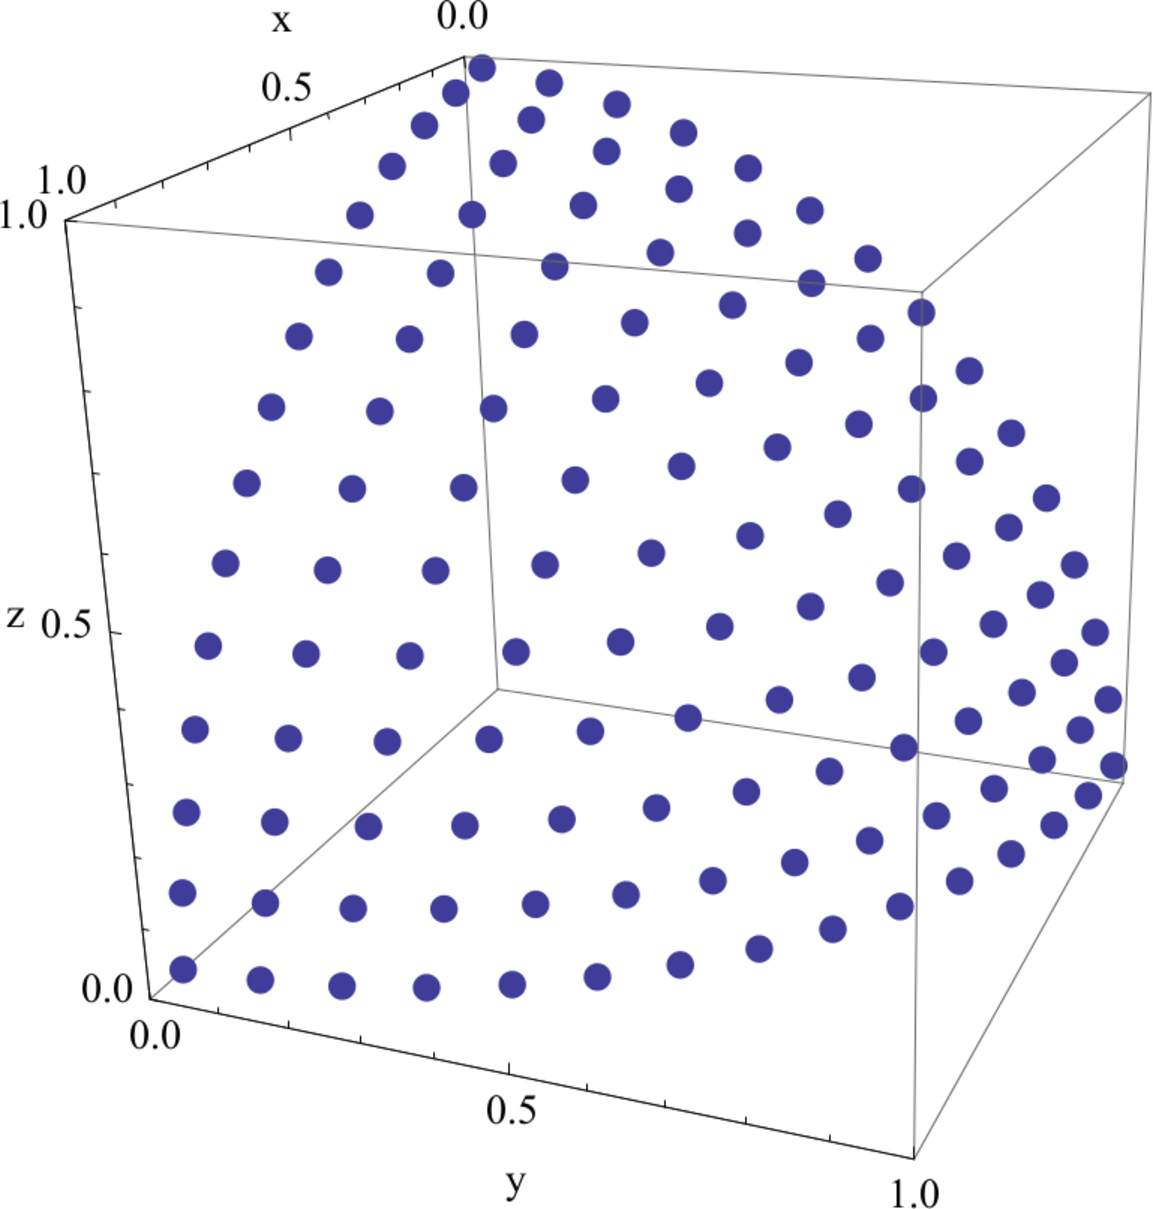
\includegraphics[scale=.375]{ordinates}
  \caption[Discrete ordinates in the first octant]{Legendre-Chebyshev
  ordinates in first octant, $N=30$}
\end{figure}

\myparagraph{Polar components}
For $l = 1,2,\ldots
N/2$, $\mu_l$ are the abscissae of the Gauss-Legendre rule, i.e. the $N/2$ positive roots of Legendre polynomial
$P_N(\mu)$. The weights are given as
$$
	w_{l}^\mu = \frac{1}{(1-\mu_l^2)\Bigl(\left.\der{P_N(\mu)}{\mu}\right\vert_{\mu_l}\Bigr)^2}.
$$

\myparagraph{Azimuthal components}
The azimuthal angle of the $i$-th direction on the $l$-th polar level is the arcus-cosine of the
$i$-th root of the Chebyshev polynomial of the first kind of degree $l$ (\cite[p.402]{weissteinCRC})\footnote{With the
ordering of the roots according to \cite{weissteinCRC}, more precisely the arcus cosine of the $l-i+1$-st root.}. That
is, for given $l = 1,2,\ldots,N$, 
$$
	\azimuthal_{l,i} = \frac{2l-2i+1}{2l}\cdot\frac{\pi}{2},\quad i = 1,2,\ldots, l.
$$
All weights on the given polar level $l$ are equal to (\cite[p.402]{weissteinCRC})
$$
	w_{l,i}^\azimuthal = \frac{\pi}{l},\quad i = 1,2,\ldots, l.
$$


\myparagraph{Complete quadrature set}
The Legendre-Chebyshev quadrature set 
$$
	\{\bomega_m,w_m\}_{M} \equiv \{\bomega_{l,i},w_{l,i}\mid l = 1,2,\ldots N,\ i = 1,2,\ldots l\}
$$ 
is defined by
\begin{equation}\label{eq:LCNset}
		\bomega_{l,i} = 
		\left[\begin{array}{c}
		\sqrt{1-\mu_l^2}\cos \azimuthal_{l,i} \\
		\sqrt{1-\mu_l^2}\sin \azimuthal_{l,i} \\
		\mu_l
	\end{array}\right],\quad
	w_{l,i} = w_{l}^\mu w_{l,i}^\azimuthal
\end{equation}
and is used in the $\SN$ module for the Hermes2D FE system (\cref{chap:hermes}). Mathematica script for generating the
quadrature points and weights is available from \alert{ref}.


\comment{
\subsubsection{}
Using the operator form of the $\SN$ equations, we can also directly verify that $\SN$ equations are not rotationally
invariant in the sense of Definition \ref{def:rotinv} in cases when the original NTE is.

\begin{theorem*}\label{thm:commut_NTE}
Let $T$ be the transport operator defined in \sref{sec:fixed-source} such that the assumptions of Theorem
\ref{thm:rotinv} are satisfied.% $RL = LR$ for all $R\in\mathrm{SO}(3)$. 
Then the corresponding $\SN$ operator
\begin{equation}\label{eq:sn_op_app}
	\Projop[S_N]\op{T}\Projop[S_N]
\end{equation}
(with $\Projop[S_N]$ defined by \eqref{eq:proj_sn}, \eqref{eq:map_SN}, \eqref{eq:map_SN_inv} and particular
ordinates and quadrature sets \mbox{$\omega = \{\bomega_n\}_{\idxset{M}}$, $\mathcal{W} = \{w_n\}_{\idxset{M}}$}
defining the patch structure $\{\Delta\bomega_m, \imath_m\}_M$) satisfies 
$$
\genop{R}\Projop[S_N]\op{T}\Projop[S_N] = \Projop[S_N]\op{T}\Projop[S_N]\genop{R}\quad \forall
\genop{R}\in\mathrm{SO}(3) $$
if and only if $M \to \infty$.
\end{theorem*}
\begin{proof}
Because of the commutativity of $T$ and $\genop{R}$, it suffices to show that $\Projop[S_N]$ commutes
with $\genop{R}$, that is 
\begin{equation}\label{eq:thm1_point}
	\genop{R} \PiSN \PihSN \psi = \PiSN \PihSN \genop{R} \psi\quad  \forall \psi \in V, 
\end{equation}
if and only if $M = \infty$.%\\[.2em] 

As in \sref{sec:opsn}, we will suppress the spatial dependence as the $\SN$ approximation concerns only the angular
dependence. For any $\psi\in V$, we have
\begin{equation*}
	\PihSN \genop{R}\psi(\bomega) = \PihSN \psi(\mat{R}^T\bomega) =
	\colset{\psi(\mat{R}^T\bomega_m)}{\idxset{M}}.
\end{equation*}
Applying $\PiSN$ thus yields a function $f_\psi \in V_{S_N}$ such that
\begin{equation}\label{eq:thm1_f}
f_\psi(\bomega) = \PiSN\PihSN \genop{R}\psi(\bomega) = \sum_{m=1}^M 
\psi(\mat{R}^T\bomega_m)\imath_m(\bomega).
\end{equation}
On the other hand, since 
$$
	\PiSN\PihSN\psi(\bomega) = \sum_{m=1}^M 
\psi(\bomega_m)\imath_m(\bomega),
$$
the rotated function $g_\psi(\bomega) = \genop{R}\PiSN\PihSN\psi(\bomega)$ is given by
\begin{equation}\label{eq:thm1_g}
g_\psi(\bomega) = \PiSN\PihSN\psi(\mat{R}^T\bomega) = \sum_{m=1}^M \psi(\bomega_m)\imath_m(\mat{R}^T\bomega)
\end{equation}
In the limit $M = \infty$, there is for each ordinate $\bomega_m$ a corresponding ordinate $\bomega_n$ such that
$$
	\bomega_m = \mat{R}^T \bomega_n,\quad \mbox{and}\quad \imath_m(\mat{R}^T\bomega) = \imath_n(\bomega)
$$ 
for any rotation matrix $\mat{R}$, so that both sums in \eqref{eq:thm1_g} and \eqref{eq:thm1_f} are equal.

On the contrary, if $M$ is finite, then also the patch areas are non-infinitesimal and there exists a rotation
$\mat{R}$ such that 
$$
	\imath_m(\mat{R}^T\bomega) = \imath_m(\bomega)\quad \forall 1 \leq m \leq M.
$$
Hence the two sums will be equal only if $\psi = \psi(\bomega)$ is constant on each patch.

In order for this equality to hold true for any $\psi \in V$ (and hence for \eqref{eq:thm1_point} to hold true), the
condition \eqref{eq:thm1_f} is also necessary.
\end{proof}

\comment{
Writing the iteration in the form
$$
\PihSN \op{L} \PiSN  \Psi_{(i+1)} = \PihSN \op{K}_{S_N} \PiSN \Psi_{(i)} + \mathrm{Q}_{S_N},
$$
we can see that propert It can be shown by Fourier analysis that
in an infinite homogeneous medium, the iteration \eqref{eq:SI} suppresses those Fourier modes with wavelengths  see also Remark \ref{rem:SI}).
\cite[Chap. 1]{Azmy1}, or \cite[Sec. II.A]{Adams})
}
}

\comment{
To summarize this subsection, we have shown that the traditional $\SN$ method that the weak form
of the $\SN$ approximation corresponds to the discontinuous Galerkin approximation in the angular domain. The $\PN$ method represents the continuous Galerkin approach.
}


\section{Approximation of spatial dependence}
\subsection{$\SN$ and $\PN$ methods}
As we have seen in the previous sections, both the $\SN$ and $\PN$ approximations lead to a system of linear
hyperbolic PDE's in spatial variables. The final approximation step typically consists of laying out a mesh  
over the spatial domain and using finite difference (FD), finite volume (FV) or finite element (FE) methods to
discretize the PDE's. 
In view of the Galerkin formulation of the $\PN$ and $\SN$ systems, it might be tempting to formulate the final
restriction to a finite dimensional subspace of $\Hp[2](X)$ in a consistent way, using as the projection target a
subspace of $\Rng\Projop[S_N]$ or $\Rng\Projop[P_N]$ spanned by a finite number of basis functions defined on $\VV$.
This can be in general done by using the finite element method, but it turns out that in current case, it is practical 
only if the $\PN$ or $\SN$ methods were applied on the second-order forms of the NTE. 

We will explain the reason for the
simpler case of the $\SN$ approximation. We will also assume that the $\SN$ equations were decoupled by the source
iteration technique and consider a single step of the process \eqref{eq:SI} with all terms on the right grouped under
the source term. Suppressing the iteration index, we may write the final system with vacuum boundary conditions as
\begin{equation}\label{eq:SNSI1}
	\mathrm{L}_{S_N} \Psi = \mathrm{Q}_{S_N},\quad\mbox{where}\quad \mathrm{L}_{S_N} \coloneqq \PihSN L \PiSN,\ \mathrm{Q}_{S_N}
	\coloneqq \PihSN q
\end{equation}
or in the expanded form as:
\begin{align}
	\bomega_m\cdot\nabla\psi_m(\br) + \sigma_t(\br)\psi_m(\br) &= q_m(\br),\quad \br \in \VV, \label{eq:SNSI2}\\
	\psi_m(\br) &= 0,\qquad \br \in \pVm[-]{m} \label{eq:SNSI2_bc}
\end{align}
for $m = 1,2,\ldots,M$,
where
$$
	\pVm[-]{m} = \{\br\in\pV : \bomega_m\cdot\bn(\br) \gtrless 0\}.
$$

Let $\mathrm{U} = [u_1,u_2,\ldots,u_M]^T$, $\mathrm{V} = [v_1,v_2,\ldots,v_M]^T$ and $\LL{\VV} =
\bigl[\Lp[2](\VV)\bigr]^M$ with the inner product 
$$
\ip{\LL{\VV}}{\mathrm{U},\mathrm{V}} = \int_{\VV}\mathrm{U}\cdot\mathrm{V}\,\d{\br} = \sum_{m=1}^M \int_{\VV} u_m(\br)
v_m(\br)\,\d{\br} = \sum_{m=1}^M (u_m, v_m)_{\Lp[2](\VV)}
$$
Further, let
$$
	\mathbb{V}(\VV) = \prod_{m=1}^M \Space_{m}(\VV),\quad \Space_{m}(\VV) = \{v\in\Lp[2](\VV): 
	\bomega_m\cdot\nabla v + \sigma_t v \in\Lp[2](\VV)\}
$$
The problem of finding a weak solution of \eqref{eq:SNSI1} can now be formulated as a problem
of finding $\Psi \in \mathbb{V}(\VV)$ with $\psi_m\vert_{\pVm[-]{m}} = 0$ such that 
\begin{equation}\label{eq:weak1}
	a(\Psi,\mathrm{V}) = f(\mathrm{V}) \quad \forall \mathrm{V}\in	\LL\VV,
\end{equation}
where
$$
	a(\Psi,\mathrm{V}) = \left(\mathrm{L}_{S_N} \Psi, \mathrm{V}\right)_{\LL\VV},\quad 
	f(\mathrm{V}) = (\mathrm{Q}, \mathrm{V})_{\LL\VV}.
$$%
\comment{
is the bilinear and linear form, respectively, associated with $\mathrm{L}_{S_N}$ by the Riesz representation theorem
and we identify $\mathrm{Q}$ on the right-hand side of \eqref{eq:SNSI1} with its Riesz representant $\mathrm{Q}\in
\mathbb{V}(\VV)$ in \eqref{eq:weak1}.}
Expanding this weak formulation and imposing the inflow boundary conditions in the weak sense by using Green's theorem,
we rewrite \eqref{eq:weak1} as
\begin{equation}\label{eq:SN_weak_system}
\left\{
\begin{aligned}
	& \sum_{m=1}^M a_{mm}(\psi_m, v_m) = \sum_{m=1}^M (q_m, v_m)_{\Lp[2](\VV)} \quad \forall
	\mathrm{V}\in\mathbb{V}(\VV),\\
	& \Psi \in \mathbb{V}(\VV)
\end{aligned}
\right.
\end{equation}
with
$$
	a_{mm}(u, v) = \int_{\VV} (-u\bomega_m\cdot\nabla v + 
	\sigma_t u v)\,\d{\br} + \int_{\pVm[+]{m}} u v\, \bomega_m\cdot\bn \d{S}.
$$


For a fixed $m$, arbitrary $v_m\in \Space_m(\VV)$ and $\mathrm{V} =
[0,\ldots,v_m,\ldots, 0]^T$, we obtain from \eqref{eq:SN_weak_system} the weak form of the
$m$-th advection-reaction equation
\begin{equation}\label{eq:SN_weak_one}
\left\{
\begin{aligned}
	& a_{mm}(\psi_m, v_m) = (q_m, v_m)_{\Lp[2](\VV)} \quad \forall v_m\in \Space_m(\VV),\\
	& \psi_m \in \Space_{m}(\VV).
\end{aligned}
\right.
\end{equation}
Let us further consider this single advection-reaction problem and suppress the index $m$. 

\subsection{Finite element method}\label{sec:FEM}
We proceed by defining a (general unstructured, quasiuniform) mesh
$\mesh = \{\elem\}$ ($\elem$ being either a simplex or a hypercube) such that $$
	\overline{\VV} = \bigcup_{\elem\in\mesh} \overline\elem
$$ where $h$ denotes
the maximum diameter of $\elem\in\mesh$. The (conforming) finite element
method restricts \eqref{eq:SN_weak_one} to a finite-dimensional subspace of $\Space$
\begin{equation}\label{eq:mesh}
	\Space_{hp} = \Rng \Projop[hp]\,u,
\end{equation}
where the projection operator may be expressed (like the $\SN$ or $\PN$ projections) as 
$\Projop[hp] = \PiHP\PihHP$, where
$$
	\PihHP : u \mapsto \mathbf{u} \in \R[N_{hp}], \quad \PiHP : \mathbf{u} \mapsto u_{hp} = \sum_{i=1}^{N_{hp}} u_i
	s_i(\br).
$$
Here for $i = 1,\ldots,N_{hp}$, $s_i \in C^0(\VV)$ are the globally continuous \textit{shape functions} generating
$\Space_{hp}$ and the mapping $\PihHP$ is defined by the choice of the finite
elements type (see \cite[Chap. 3]{dolfin1}).
The classical choice of shape functions are the piecewise polynomial functions, giving rise to the approximation
subspace
\begin{equation}\label{eq:space}
	\Space_{hp} = \{v_{hp} \in C^0(\VV): \left. v_{hp}\right\vert_{\elem} \circ\, \mathfrak{r} \in
	\mathcal{P}_p(\hat{\elem}),\ \elem\in\mesh
	\}
\end{equation}
where $\hat{\elem}$ is the reference unit hypercube or simplex, $\mathfrak{r} : \elem \to \hat{\elem} $
is the standard reference mapping and $\mathcal{P}_p(\hat{\elem})$ is the space of polynomials of degree up to $p$
(tensor product polynomials in case of $\elem$ being a hypercube).

As a result of the restriction of \eqref{eq:SN_weak_one} to $\Space_{hp}$, we obtain for $u,v\in\Space$
\begin{equation}\label{eq:aaa}
	a(u_{hp}, v_{hp}) = a(\Projop[hp]u, \Projop[hp]v) = a(\PiHP \mathbf{u}, \PiHP \mathbf{v}) =
	(\mathbf{A}\mathbf{u})^T\mathbf{v}
\end{equation}
where
$$
	[\mat{A}]_{ij} = (\mat{A}\mat{e}_i)^T\mat{e}_j = a(s_i, s_j) 
$$
and analogously 
$$
	(q,\Projop[hp] v) = \mat{b}^T \mat{v}, \quad [\mat{b}]_i = (q, s_i)_{\Lp[2](\VV)};
$$
that is, the algebraic system
$$
	\mathbf{A}\mathbf{u} = \mathbf{b},\quad \mathbf{A} \in \R[N_{hp}\times N_{hp}], \ \mat{u},\mat{b} \in \R[N_{hp}].
$$


\noindent Returning back to the general case with $m = 1,\ldots,M$, the matrix $\mathbf{A}$
would form the $mm$ block in the global $\SN$ matrix (restriction of eq. \eqref{eq:weak1} to $\prod_{m} \Space_{m,hp}(\VV)$).  

By this construction, $\Space_{hp} \subset \Space$ \footnote{provided that \eqref{eq:mesh} holds, which is often
violated by the inability to precisely capture the geometrical boundaries; however, we will not consider this
\textit{variational crime} here} and we may consider the above procedure as another restriction of the NTE following its restriction to $V_{SN}$.
The finite dimensional subspace in which we are looking for the solution has dimension $N_{hp} \times M \times G$ (if we also consider the multigroup discretization of energy).

Equations of type \eqref{eq:SN_weak_one} have been studied extensively in the past (see e.g. \cite{hartmann} and
references therein) and it is well known that the bilinear form in \eqref{eq:SN_weak_one} is not coercive on
$\Space_m(\VV)$. Namely, there exists $\alpha > 0$ such that for any $v \in \Space_m(\VV)$,
\begin{equation}\label{eq:unstable}
	a_{mm}(v,v) \geq \alpha \norm[{\Lp[2](\VV)}]{v}^2 + \frac{1}{2}\int_{\pV} \abs{\bomega_m\cdot\bn} v^2 \,\d{S},
\end{equation}
while the norm on $\Space_m(\VV)$ is given by
$$
	\norm[{\Space_m(\VV)}]{v}^2 = \norm[{\Lp[2](\VV)}]{\bomega_m\cdot\nabla v}^2 + \norm[{\Lp[2](\VV)}]{v}^2 +
	\int_{\pV} \abs{\bomega_m\cdot\bn} v^2 \,\d{S}. 
$$
As coercivity is preserved by restricting to a subspace, this property may be expected to be reflected by the
discretization described above. Indeed, if the exact solution is not sufficiently smooth (and it is generally not in
practice) unstable results with spurious oscillations arise because the directional derivative is uncontrolled by the
right-hand side of \eqref{eq:unstable}.

\comment{
In the case of the $\SN$ approximation, the approach traditionally favored by the nuclear engineering community
uses the source iteration technique to decouple the system into simple advection-reaction equations,
each of which is then solved by a \textit{transport sweep} from inflow to outflow boundaries of mesh cells. The finite volume method is used to link
the mesh cells through cell-averaged and interface unknowns. Without fission and scattering (i.e., the integral term
$\op{K}$ in \eqref{eq1op}) and reflective boundaries (\eqref{eq:nte3}), the system is already decoupled and only one
sweep for each direction is sufficient to determine $\op{L}^{-1}$ and hence the solution. Otherwise, the
iteration as described in \sref{sec:SI} is required.
}
\comment{
Similarly to the explicit schemes for usual time-dependent advection-reaction problems, this direction-sweeping scheme
requires careful choice of numerical approximation of interface unknowns to ensure stability (restricting and
intertwinning the angular and spatial resolution). An alternative, attractive in particular when an unstructured spatial
mesh is used (and even more in three dimensions), is the implicit solution of of the angularly discretized system. This
is also the method of choice for the $\PN$ system, where diagonalization of the advection matrices for each differently
oriented cell interface would be required for the sweeping procedure. However, the stability constraints do not
disappear completely -- in order not to introduce excessive oscillations into the solution, a stable spatial
discretization must be used to obtain the algebraic system. 
}
\comment{
In view of the Galerkin formulation of the $\PN$ and $\SN$ systems, it might be tempting to formulate the final
restriction to a finite dimensional subspace of $\Hp[2](X)$ in a consistent way, using as the projection target a
finite-dimensional subspace of $\Rng\Projop[S_N]$ or $\Rng\Projop[P_N]$. This can be in general done by using the
finite element method, but it turns out that in current case, it is possible only when the $\PN$ or $\SN$ methods were
applied on the second-order forms of the NTE. 
}
\comment{
We will explain the reason for the simpler case of the $\SN$
approximation. 

To this end, let us consider the $\SN$ operator equations \eqref{eq:sn_op} in the Hilbert space 
$$
	\mathbb{V}(\VV) = \bigl[\Space\bigr]^K
$$
We will use the following notation for the operator from \eqref{eq:sn_op}:
$$
	\mat{T}_{S_N} = \PihSN (L-K) \PiSN
$$ 
and define inner product of vector functions $\mathrm{U} = [u_1,u_2,\ldots,u_M]^T$, $\mathrm{V} =
[v_1,v_2,\ldots,v_M]^T$ in $\mathbb{V}$ by 
$$
\ip{\mathbb{V}}{\mathrm{U},\mathrm{V}} = \int_{\VV}\mathrm{U}\cdot\mathrm{V} = \sum_{n=1}^M \int_{\VV} u_n(\br)
v_n(\br)\,\d{\br}.
$$
The problem of solving equations \eqref{eq:sn_op} can now be formulated as a problem
to find $\Psi \in \Space$ such that
\begin{equation}\label{eq:weak1}
	a(\Psi,\Theta) = (\mathrm{Q}, \Theta)_\mathbb{V} \quad \forall \Theta\in \mathbb{V}(\VV),
\end{equation}
where
$$
	a(\Psi,\Theta) \coloneqq \left(\mat{L}_{S_N} \Psi, \Theta\right)_\mathbb{V}
$$
and we identify $\mathrm{Q}$ on the right-hand side of \eqref{eq:sn_op} with its Riesz
representant $\mathrm{Q}\in \mathbb{V}(\VV)$ in \eqref{eq:weak1}.
}

\comment{
In the case of the finite element method, for example, it is well known that the approximation of the
solution of an advection-reaction PDE by piecewise continuous functions (i.e., the continuous Galerkin method) is not
stable and allows arbitrarily large oscillations. 
}

\subsubsection{Discontinuous Galerkin method}\label{sec:DGM}
To circumvent this issue, one approach is to give up conformity and define an appropriate approximation space on which
the restricted bilinear form can be shown to be coercive. This leads to the \textit{discontinuous Galerkin method}
of order $p$, shortly DG(p), where the shape functions are still polynomials of degree up to $p$ on each element, but
are not required to be globally continuous:
$$
\Space_{hp}^{dg} = \{v_{hp} \in \Lp[2](\VV): \left. v_{hp}\right\vert_{\elem} \circ\, \mathfrak{r} \in
	\mathcal{P}_p(\hat{\elem}),\ \elem\in\mesh
	\}.
$$
Because of the insufficient smoothness of functions from $\Space_{hp}^{dg}$, the Green's theorem used for obtaining the
weak form must be applied element-wise, leading to the formulation (for a particular direction $\bomega\in\omega$)
$$
	\sum_{\elem\in\mesh}\int_{\elem} (-u_{hp}\bomega\cdot\nabla v_{hp} + 
	\sigma_t u_{hp} v_{hp})\,\d{\br} + \sum_{e\not\subset\pV[-]}\int_{e} \langle\bomega u_{hp}\rangle\cdot \jump{v_{hp}}\,
	\d{S} = \int_{\VV} q v_{hp}\,\d{\br} 
$$
where $e$ denotes subsequently all faces of all elements $\elem\in\mesh$ (both interior and those coinciding with
segments of $\pV$) and for each face
$$
	\jump{v_{hp}} = \pw{v_{hp}\bn^- + v_{hp}\bn^+}{for $e\not\subset\pV$}{v_{hp}\bn}{for $e\subset\pV$}
$$
with $\bn^{\pm}$ the outer normal of $\elem^+$ and $\elem^-$, respectively, where $e = \elem^- \cap \elem^+$.
There are several ways of approximating $\bomega u_{hp}$ by $\{\bomega u_{hp}\}$ (called \textit{numerical flux}), the
simplest stable approximation being the \textit{upwind numerical flux}:
$$
	\langle\bomega u_{hp}\rangle = 
	\begin{cases}
		\bomega u_{hp}^-, & \bomega\cdot\bn^- > 0,\\
		\bomega u_{hp}^+, & \bomega\cdot\bn^- < 0,\\
		\bomega \frac{u_{hp}^- + u_{hp}^+}{2}, & \bomega\cdot\bn^- = 0
	\end{cases}
$$
where $u_{hp}^{\pm}$ denotes the trace $u_{hp}\vert_e$ taken from $\elem^+$ and $\elem^-$, respectively. We refer e.g.
to \cite{hartmann} for further details.

Another approach leaves the approximation space conforming (continuous), but modifies directly the bilinear form
(typically by adding some artificial diffusion). This leads to stabilized continuous Galerkin methods (in which
the bilinear form becomes dependent on mesh parameter $h$). We refer to \cite{kanschat} for the application of a
particular conforming stabilized method -- the streamline-upwind Petrov Galerkin method -- and further discussion about
the discontinuous Galerkin method.

\subsection{Diffusion approximation}\label{sec:diffusion_weak}

Much simpler situation arises in the spatial discretization of the diffusion equation \eqref{eq:diffusion} with boundary
conditions \eqref{eq:diffusion_bc}. In this case, the original problem is posed in the usual Sobolev space $H^1(\VV)$: 
Find $u\in H^1(\VV)$ such that
\begin{equation}\label{eq:dif_bil_ex}
	a(u,v) = f(v)	\quad	\forall v\in H^1(\VV)
\end{equation}
where 
$$ 
	a(u,v) = (D\nabla u, \nabla v)_{\Lp[2](\VV)} + (\Sigma u, v)_{\Lp[2](\VV)} + (\gamma u, v)_{\Lp[2](\pV)},\quad
	f(v) = (q,v)_{\Lp[2](\VV)}.
$$
(with $\Sigma = \sigma_t(\br) - \sigma_{s0}(\br)  - \nu\sigma_f(\br)$, $D$ defined in eq. \eqref{eq:diffusion} and
$\gamma$ in \eqref{eq:diffusion_bc}).
Under the subcriticality conditions, the bilinear form $a$ is bounded and coercive on $H^1(\VV)$ (even in the multigroup
case -- see \cite[Chap. VII]{DautrayLions2}). By using the finite element method as described
above with the approximation space \eqref{eq:space}, an algebraic system
\begin{equation}\label{eq:syst}
	\mat{A}\mat{u} = \mat{b}
\end{equation}
with sparse, symmetric, positive definite (in the mono-energetic case) matrix $\mat{A}$ is obtained, amenable to
solution by standard numerical methods.


\subsection{On origin of errors in the FE approximation}
Let us finish this section by recalling a simple, but very important connection between the above described finite
element discretization and solution of \eqref{eq:syst}. Even though the
analysis is done here for the case of the diffusion approximation with symmetric and positive definite system
\eqref{eq:syst}, keeping in mind its conclusion is equally important for finite-element discretizations of the other
models as well.

As before, after restricting to $\Space_{hp} \subset
H^1(\VV)$ we get the approximate problem:
Find $u_{hp}\in \Space_{hp}$ such that
$$
	a(u_{hp}, v_{hp}) = f(v_{hp}) \quad \forall v_{hp} \in \Space_{hp}
$$
(where $u_{hp} = \Projop[hp] u$, $v_{hp} = \Projop[hp] v$). Subtracting from \eqref{eq:dif_bil_ex}, we obtain the
well-known \textit{Galerkin orthogonality} property:
$$
	a(u - u_{hp}, v_{hp}) = 0	\quad \forall v_{hp}\in \Space_{hp},
$$
which characterizes the \textit{discretization error}. In practice, it is impossible to solve the system \eqref{eq:syst}
exactly, so suppose that we have obtained after $n$ steps of a suitable iterative method the solution $\mat{u}_{(n)}$,
such that the \textit{algebraic error} $\mat{u} - \mat{u}_{(n)}$ is nontrivial. By applying $\PihHP$ to the algebraic
error, we obtain the representation of that error in $\Space_{hp}$: 
$$
	u_{hp} - u_{hp}^{(n)} \in \Space_{hp}
$$
(where we temporarily shifted the iteration index to improve readability).
Hence, by decomposing the total error as
$$
	u - u_{hp}^{(n)} = (u-u_{hp}) + (u_{hp}-u_{hp}^{(n)})
$$
and applying Galerkin orthogonality, we find that
$$
	a(u - u_{hp}^{(n)}) = a(u-u_{hp}) + a(u_{hp}-u_{hp}^{(n)}).
$$
Also by noticing that 
$$
	a(u_{hp}-u_{hp}^{(n)}) = \bigl(\mat{u} - \mat{u}_{(n)}\bigr)^T\mat{A}\bigl(\mat{u} - \mat{u}_{(n)}\bigr) =
	\norm[\mat{A}]{\mat{u} - \mat{u}_{(n)}} $$
(see \eqref{eq:aaa})
we get the fundamental representation of the energy norm of the total error as a sum of the discretization error and
algebraic error contributions:
$$
	a(u - u_{hp}^{(n)}) = a(u-u_{hp}) + \norm[\mat{A}]{\mat{u} - \mat{u}_{(n)}}.
$$
In theory, the first part could be controlled by a suitable $hp$-adaptivity process, while for the latter, using the
methods that are based on minimization of the $\mat{A}$-norm of error (the CG method among the Krylov subspace methods,
or the smoothed aggregation multigrid method, as we demonstrate in App. \ref{app:multigrid}). However, striking the
balance between the two contributions and determining optimal stopping criteria for the algebraic solution methods accordingly is an important area of active research (notably in the case when the latter is further split to account for rounding errors of 
computers) and we refer to paper \cite{Arilie} and its extensive list of references for further details.
\comment{
Even in this case, with the simplest angular discretization, the system of linear algebraic equations is -- given the
complicated geometry and material arrangement of realistic problems -- very large. In realistic cases, it is
computationally infeasible to resolve all local features of the solution by a uniform mesh and some sort of adaptivity 
is needed. It is typically driven by employed. In some cases (typically in engineering application like the simulation
of heterogeneous nuclear reactor cores), the long-term experience may be used to create the mesh by hand using well-established geometry and mesh generation software like the commercial CUBIT (\cite{CUBIT}) or the open-source GMSH (\cite{GMSH}). When the a-priori knowledge of important solution features is not
available, some sort of automatic adaptivity is needed, which we will discuss in a broader sense (including also the
adaptivity in angular domain) in the following section.

As a final note, we would like to remark that solution of the algebraic systems 
}
\section{Adaptivity}
In real applications, automatic adaptivity of the discrete phase space is usually needed to obtain sufficiently accurate
results sufficiently fast. Except for the scheme described in the Ph.D. thesis of H. Park \cite{Park} -- a rare case of 
 coupled angular and spatial adaptivity -- all literature available to the author describes schemes where angular and
spatial adaptivity is performed separately (and there is none about adaptivity with respect to the energetic variable). 
In the context of the $\PN$ method, there are examples where the order of the spherical harmonic expansion is varied 
throughout the spatial domain (see e.g. \cite{Ackroyd2}) based on material properties and physical reasoning. Properties
of spherical wavelets have been used in \cite{Buchan} to drive automatic selection of the order of the expansion  (in
this case with respect to the wavelet interpolation basis of $\Lp[2](\Sphere)$ instead of the spherical harmonics basis)
based on the increasing size of expansion coefficients corresponding to wavelets supported over underresolved areas of 
$\Sphere$. Angular adaptivity in the $\SN$ approximation (i.e., adaptive control of the number of discrete ordinates in 
local areas on the sphere) is described in \cite{Jarrell}.

More widespread use has found the adaptivity in spatial domain, using techniques developed for finite element
approximations of general hyperbolic systems. They are usually used in DG $\SN$ methods, see e.g.
\cite{Fournier,Duo,ragusa2010two} for adaptivity based on a-posteriori estimation of global $\Lp[2]$ norm of solution
error or \cite{LathouwersGoal, Wang2} for a method based on goal oriented adaptivity. Spatial adaptivity for the
standard $\PN$ approximation is not used as widely, probably because the approximation itself is not so widely used for
larger scale calculations. However, $\PN$ approximations of the second-order forms of NTE (introduced in
\sref{sec:L2}) lead to a system of second-order PDEs for which many usual a-posteriori estimates for elliptic 
PDEs have been successfully applied. In particular, spatial adaptivity for the diffusion and simplified $\PN$
approximations has been widely used in the past.
 
The discontinuous Galerkin framework doesn't impose any constraints on the solution
continuity accross elements and allows the solution to be represented by completely different functions on each element.
As such, it is well-suited for implementing both the mesh refinement and polynomial order variation procedure, paving a
way for hp-adaptive FE solution.
Nevertheless, all the references above are employing h-adaptivity where the mesh is refined with fixed polynomial
approximation degree $p$. Prevalence of h-adaptivity and use of $p=1$ (linear) finite element spaces is caused partly
by the difficulty of implementation of an hp-adaptive FE code itself, partly by the fear of the well known limited
regularity of the exact solution of \eqref{eq1} even for smooth input data\footnote{By the method of characteristics, we
can expect the angular fluxes $\angflux(\cdot,\bomega)$ to be differentiable in the direction of $\bomega$, but not in
any other direction. As shown in \cite{Johnson}, the scalar fluxes, i.e. integrals of $\angflux$ over $\Sphere$, belong
at most to $H^{3/2-\epsilon}(\VV)$ where $0 < \epsilon \ll 1$ and $H^{k}(\VV)$ denotes the Sobolev space of fractional
order $k$ (e.g., \cite[Sec. 9.2]{demkowicz}).}.
However, similarly to the experience with hp-adaptive methods in different fields, the limitation of asymptotic
convergence rate (as $h\to 0$ where $h$ is the diameter of the largest element in the mesh) dictated by a-priori error
estimates involving solution regularity typically doesn't appear until very late in the mesh refinement process or at
all (\cite{wang2009convergence}). Hence, utilizing higher order approximations still makes sense to accelerate
pre-asymptotic convergence rate as much as possible (for an attempt to use hp-adaptivity with DG $\SN$ methods -- to
author's knowledge first of its kind, see \cite{FournierDGHP}). Implementation of an $\SN$ solver in the general hp-FEM
framework Hermes (see \cref{chap:hermes}), could be seen as a first step for future investigations in this
direction.



% REGULARITY


  

\comment{

\subsubsection{Solution of the associated algebraic systems}

Nevertheless, both approaches lead to very large systems (easily of the order of $10^8$ even for a crude energetic
discretization), often ill-conditioned as a result of highly irregular material properties or meshes
(particularly when automatic mesh refinement is employed). Using even the advanced sparse direct solvers like
UMFPACK or MUMPS (\cite{UMFPACK,MUMPS}) to solve such systems is not practical.
Moreover, it is intuitively obvious and easily proved (see e.g. \cite{Arioli}) that the total approximation error is
given by the sum of di

Moreover, there are cases (typically
in engineering applications like the simulation of heterogeneous nuclear reactor cores) where it is common to create
initial spatial mesh by some specialized CAD and mesh-generation system based on the long-time operating experience. ,
The need to resolve a complicated dependence on 6 independent variables may easily result in systems with

Robust solvers that Also, because of the possibly highly heterogeneous domains with large jumps in material coefficients
between subdomains, conditioned
}